\documentclass[a4paper]{book}
\usepackage{a4wide}
\usepackage{makeidx}
\usepackage{fancyhdr}
\usepackage{graphicx}
\usepackage{multicol}
\usepackage{float}
\usepackage{textcomp}
\usepackage{alltt}
\usepackage{times}
\usepackage{ifpdf}
\ifpdf
\usepackage[pdftex,
            pagebackref=true,
            colorlinks=true,
            linkcolor=blue,
            unicode
           ]{hyperref}
\else
\usepackage[ps2pdf,
            pagebackref=true,
            colorlinks=true,
            linkcolor=blue,
            unicode
           ]{hyperref}
\usepackage{pspicture}
\fi
\usepackage[utf8]{inputenc}
\usepackage{doxygen}
\makeindex
\setcounter{tocdepth}{3}
\renewcommand{\footrulewidth}{0.4pt}
\begin{document}
\begin{titlepage}
\vspace*{7cm}
\begin{center}
{\Large Nessie, reconocedor óptico de texto en recortes de prensa escrita \\[1ex]\large 1.0 }\\
\vspace*{1cm}
{\large Generated by Doxygen 1.5.6}\\
\vspace*{0.5cm}
{\small Mon Oct 6 12:30:24 2008}\\
\end{center}
\end{titlepage}
\clearemptydoublepage
\pagenumbering{roman}
\tableofcontents
\clearemptydoublepage
\pagenumbering{arabic}
\chapter{Directory Hierarchy}
\section{Directories}
This directory hierarchy is sorted roughly, but not completely, alphabetically:\begin{CompactList}
\item \contentsline{section}{inc}{\pageref{dir_ef15eccf5bd9eca446a41a18c57ac0fd}}{}
\item \contentsline{section}{src}{\pageref{dir_f108b8e716a38a781a23bf0e62a4b450}}{}
\end{CompactList}

\chapter{Data Structure Index}
\subsection{Data Structures}
Here are the data structures with brief descriptions:\begin{CompactList}
\item\contentsline{section}{\hyperlink{class_clip}{Clip} (Press clip where the recognizer has to extract the text from )}{\pageref{class_clip}}{}
\item\contentsline{section}{\hyperlink{class_clip_location}{ClipLocation} (Location of a press clip inside a newspaper page )}{\pageref{class_clip_location}}{}
\item\contentsline{section}{\hyperlink{class_nessie_exception}{NessieException} (Exception raised by a Nessie OCR object )}{\pageref{class_nessie_exception}}{}
\item\contentsline{section}{\hyperlink{class_preprocessor}{Preprocessor} (\hyperlink{class_preprocessor}{Preprocessor} of the OCR process )}{\pageref{class_preprocessor}}{}
\item\contentsline{section}{\hyperlink{class_recognizer}{Recognizer} (Manager of the whole OCR process )}{\pageref{class_recognizer}}{}
\item\contentsline{section}{\hyperlink{class_segmenter}{Segmenter} (\hyperlink{class_segmenter}{Segmenter} of the OCR process )}{\pageref{class_segmenter}}{}
\item\contentsline{section}{\hyperlink{class_shape}{Shape} (The shape of a character in a press clip )}{\pageref{class_shape}}{}
\item\contentsline{section}{\hyperlink{class_statistics}{Statistics} (Statistical data regarding the text recognition process )}{\pageref{class_statistics}}{}
\item\contentsline{section}{\hyperlink{class_text}{Text} (\hyperlink{class_text}{Text} extracted by the recognizer )}{\pageref{class_text}}{}
\end{CompactList}

\chapter{File Index}
\section{File List}
Here is a list of all documented files with brief descriptions:\begin{CompactList}
\item\contentsline{section}{\textbf{Classifier.cpp} }{\pageref{_classifier_8cpp}}{}
\item\contentsline{section}{\textbf{Classifier.h} }{\pageref{_classifier_8h}}{}
\item\contentsline{section}{\hyperlink{_clip_8cpp}{Clip.cpp} (Implementation of class \hyperlink{class_clip}{Clip} )}{\pageref{_clip_8cpp}}{}
\item\contentsline{section}{\hyperlink{_clip_8h}{Clip.h} (Declaration of class \hyperlink{class_clip}{Clip} )}{\pageref{_clip_8h}}{}
\item\contentsline{section}{\hyperlink{_colorspace_8h}{Colorspace.h} (Declaration of enumeration Colorspace )}{\pageref{_colorspace_8h}}{}
\item\contentsline{section}{\textbf{FeatureVector.cpp} }{\pageref{_feature_vector_8cpp}}{}
\item\contentsline{section}{\textbf{FeatureVector.h} }{\pageref{_feature_vector_8h}}{}
\item\contentsline{section}{\textbf{loadPDF.cpp} }{\pageref{load_p_d_f_8cpp}}{}
\item\contentsline{section}{\textbf{main.cpp} }{\pageref{main_8cpp}}{}
\item\contentsline{section}{\hyperlink{_nessie_exception_8cpp}{NessieException.cpp} (Implementation of class \hyperlink{class_nessie_exception}{NessieException} )}{\pageref{_nessie_exception_8cpp}}{}
\item\contentsline{section}{\hyperlink{_nessie_exception_8h}{NessieException.h} (Declaration of class \hyperlink{class_nessie_exception}{NessieException} )}{\pageref{_nessie_exception_8h}}{}
\item\contentsline{section}{\textbf{Partitioner.cpp} }{\pageref{_partitioner_8cpp}}{}
\item\contentsline{section}{\textbf{Partitioner.h} }{\pageref{_partitioner_8h}}{}
\item\contentsline{section}{\hyperlink{_pixel_8cpp}{Pixel.cpp} (Implementation of class \hyperlink{class_pixel}{Pixel} )}{\pageref{_pixel_8cpp}}{}
\item\contentsline{section}{\hyperlink{_pixel_8h}{Pixel.h} (Declaration of class \hyperlink{class_pixel}{Pixel} )}{\pageref{_pixel_8h}}{}
\item\contentsline{section}{\hyperlink{_preprocessor_8cpp}{Preprocessor.cpp} (Implementation of class \hyperlink{class_preprocessor}{Preprocessor} )}{\pageref{_preprocessor_8cpp}}{}
\item\contentsline{section}{\hyperlink{_preprocessor_8h}{Preprocessor.h} (Declaration of class \hyperlink{class_preprocessor}{Preprocessor} )}{\pageref{_preprocessor_8h}}{}
\item\contentsline{section}{\textbf{Recognizer.cpp} }{\pageref{_recognizer_8cpp}}{}
\item\contentsline{section}{\textbf{Recognizer.h} }{\pageref{_recognizer_8h}}{}
\item\contentsline{section}{\hyperlink{_rgb_color_8cpp}{RgbColor.cpp} (Implementation of struct \hyperlink{struct_rgb_color}{RgbColor} )}{\pageref{_rgb_color_8cpp}}{}
\item\contentsline{section}{\hyperlink{_rgb_color_8h}{RgbColor.h} (Declaration of struct \hyperlink{struct_rgb_color}{RgbColor} )}{\pageref{_rgb_color_8h}}{}
\item\contentsline{section}{\textbf{Shape.cpp} }{\pageref{_shape_8cpp}}{}
\item\contentsline{section}{\textbf{Shape.h} }{\pageref{_shape_8h}}{}
\item\contentsline{section}{\hyperlink{_statistics_8cpp}{Statistics.cpp} (Implementation of structure \hyperlink{struct_statistics}{Statistics} )}{\pageref{_statistics_8cpp}}{}
\item\contentsline{section}{\hyperlink{_statistics_8h}{Statistics.h} (Declaration of struct \hyperlink{struct_statistics}{Statistics} )}{\pageref{_statistics_8h}}{}
\item\contentsline{section}{\hyperlink{_text_8cpp}{Text.cpp} (Implementation of class \hyperlink{class_text}{Text} )}{\pageref{_text_8cpp}}{}
\item\contentsline{section}{\hyperlink{_text_8h}{Text.h} (Declaration of class \hyperlink{class_text}{Text} )}{\pageref{_text_8h}}{}
\item\contentsline{section}{\hyperlink{_word_rate_8h}{WordRate.h} (Declaration of custom type WordRate )}{\pageref{_word_rate_8h}}{}
\end{CompactList}

\chapter{Directory Documentation}
\hypertarget{dir_ef15eccf5bd9eca446a41a18c57ac0fd}{
\section{inc/ Directory Reference}
\label{dir_ef15eccf5bd9eca446a41a18c57ac0fd}\index{inc/ Directory Reference@{inc/ Directory Reference}}
}




\nopagebreak
\begin{figure}[H]
\begin{center}
\leavevmode
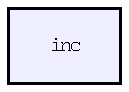
\includegraphics[width=49pt]{dir_ef15eccf5bd9eca446a41a18c57ac0fd_dep}
\end{center}
\end{figure}
\subsection*{Files}
\begin{CompactItemize}
\item 
file \textbf{Classifier.hpp}
\item 
file \hyperlink{_clip_8hpp}{Clip.hpp}
\begin{CompactList}\small\item\em Declaration of the class \hyperlink{class_clip}{Clip}. \item\end{CompactList}

\item 
file \hyperlink{_clip_location_8hpp}{ClipLocation.hpp}
\begin{CompactList}\small\item\em Declaration of the class \hyperlink{class_clip_location}{ClipLocation}. \item\end{CompactList}

\item 
file \textbf{FeatureVector.hpp}
\item 
file \hyperlink{_nessie_exception_8hpp}{NessieException.hpp}
\begin{CompactList}\small\item\em Declaration of the class \hyperlink{class_nessie_exception}{NessieException}. \item\end{CompactList}

\item 
file \hyperlink{_pixel_8hpp}{Pixel.hpp}
\begin{CompactList}\small\item\em Declaration of the custom type Pixel. \item\end{CompactList}

\item 
file \hyperlink{_preprocessor_8hpp}{Preprocessor.hpp}
\begin{CompactList}\small\item\em Declaration of the class \hyperlink{class_preprocessor}{Preprocessor}. \item\end{CompactList}

\item 
file \hyperlink{_recognizer_8hpp}{Recognizer.hpp}
\begin{CompactList}\small\item\em Declaration of the class \hyperlink{class_recognizer}{Recognizer}. \item\end{CompactList}

\item 
file \hyperlink{_segmenter_8hpp}{Segmenter.hpp}
\begin{CompactList}\small\item\em Declaration of the class \hyperlink{class_segmenter}{Segmenter}. \item\end{CompactList}

\item 
file \hyperlink{_shape_8hpp}{Shape.hpp}
\begin{CompactList}\small\item\em Declaration of the class \hyperlink{class_shape}{Shape}. \item\end{CompactList}

\item 
file \hyperlink{_statistics_8hpp}{Statistics.hpp}
\begin{CompactList}\small\item\em Declaration of the class \hyperlink{class_statistics}{Statistics}. \item\end{CompactList}

\item 
file \hyperlink{_text_8hpp}{Text.hpp}
\begin{CompactList}\small\item\em Declaration of the class \hyperlink{class_text}{Text}. \item\end{CompactList}

\end{CompactItemize}

\hypertarget{dir_f108b8e716a38a781a23bf0e62a4b450}{
\section{src/ Directory Reference}
\label{dir_f108b8e716a38a781a23bf0e62a4b450}\index{src/ Directory Reference@{src/ Directory Reference}}
}




\nopagebreak
\begin{figure}[H]
\begin{center}
\leavevmode
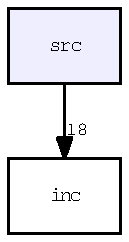
\includegraphics[width=49pt]{dir_f108b8e716a38a781a23bf0e62a4b450_dep}
\end{center}
\end{figure}
\subsection*{Files}
\begin{CompactItemize}
\item 
file \textbf{Classifier.cpp}
\item 
file \hyperlink{_clip_8cpp}{Clip.cpp}
\begin{CompactList}\small\item\em Implementation of the class \hyperlink{class_clip}{Clip}. \item\end{CompactList}

\item 
file \hyperlink{_clip_location_8cpp}{ClipLocation.cpp}
\begin{CompactList}\small\item\em Implementation of the class \hyperlink{class_clip_location}{ClipLocation}. \item\end{CompactList}

\item 
file \textbf{FeatureVector.cpp}
\item 
file \hyperlink{main_8cpp}{main.cpp}
\begin{CompactList}\small\item\em Implementation of a command line program for testing purposes. \item\end{CompactList}

\item 
file \hyperlink{_nessie_exception_8cpp}{NessieException.cpp}
\begin{CompactList}\small\item\em Implementation of the class \hyperlink{class_nessie_exception}{NessieException}. \item\end{CompactList}

\item 
file \hyperlink{_preprocessor_8cpp}{Preprocessor.cpp}
\begin{CompactList}\small\item\em Implementation of the class \hyperlink{class_preprocessor}{Preprocessor}. \item\end{CompactList}

\item 
file \hyperlink{_recognizer_8cpp}{Recognizer.cpp}
\begin{CompactList}\small\item\em Implementation of the class \hyperlink{class_recognizer}{Recognizer}. \item\end{CompactList}

\item 
file \hyperlink{_segmenter_8cpp}{Segmenter.cpp}
\begin{CompactList}\small\item\em Definition of the class \hyperlink{class_segmenter}{Segmenter}. \item\end{CompactList}

\item 
file \hyperlink{_shape_8cpp}{Shape.cpp}
\begin{CompactList}\small\item\em Implementation of the class \hyperlink{class_shape}{Shape}. \item\end{CompactList}

\item 
file \hyperlink{_statistics_8cpp}{Statistics.cpp}
\begin{CompactList}\small\item\em Implementation of the class \hyperlink{class_statistics}{Statistics}. \item\end{CompactList}

\item 
file \hyperlink{_text_8cpp}{Text.cpp}
\begin{CompactList}\small\item\em Implementation of the class \hyperlink{class_text}{Text}. \item\end{CompactList}

\end{CompactItemize}

\chapter{Data Structure Documentation}
\hypertarget{class_clip}{
\section{Clip Class Reference}
\label{class_clip}\index{Clip@{Clip}}
}
{\tt \#include $<$Clip.h$>$}

Collaboration diagram for Clip:\nopagebreak
\begin{figure}[H]
\begin{center}
\leavevmode
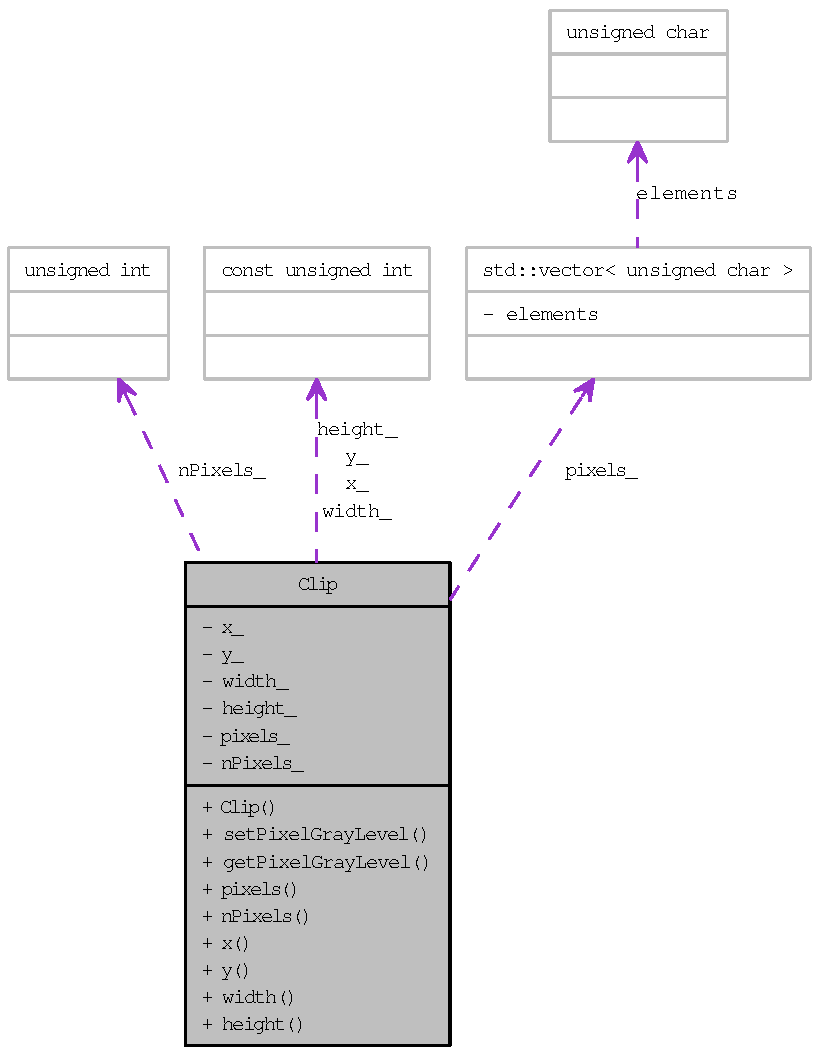
\includegraphics[width=400pt]{class_clip__coll__graph}
\end{center}
\end{figure}


\subsection{Detailed Description}
Press clip where the recognizer has to extract the text from. 

This class manages the press clip where the recognizer has to extract the text, loading it with the Magick++ utilities. The press clip is an image that may come in several formats, such JPEG, PDF, PNG, etc. The ImageMagick library provides an abstraction layer to keep the code independent from the format.

The idea behind this class is to encapsulate all the interactions with the Magick++ API, so that the rest of the classes have a unified way to work with the original image.

\begin{Desc}
\item[See also:]\hyperlink{class_pixel}{Pixel}, \hyperlink{_colorspace_8h_7a7e24cdb2a27271343f0adceff89f65}{Colorspace}\end{Desc}
\begin{Desc}
\item[Author:]Eliezer Talón (\href{mailto:elitalon@gmail.com}{\tt elitalon@gmail.com}) \end{Desc}
\begin{Desc}
\item[Date:]2008-09-29 \end{Desc}


Definition at line 37 of file Clip.h.\subsection*{Public Member Functions}
\begin{CompactItemize}
\item 
\hyperlink{class_clip_f8f4312cce2d38d61ce370912e9e7e4a}{Clip} (Image image, unsigned int xOrigin, unsigned int yOrigin, unsigned int height, unsigned int width)
\begin{CompactList}\small\item\em Constructor. \item\end{CompactList}\item 
\hyperlink{class_clip_88647ed65e3482b5e0533ec98667b0fa}{$\sim$Clip} ()
\begin{CompactList}\small\item\em Destructor. \item\end{CompactList}\item 
Image \hyperlink{class_clip_f4500103f1babcf2b9283eaffc6af96a}{image} ()
\begin{CompactList}\small\item\em Returns the current Image object. \item\end{CompactList}\item 
unsigned int \hyperlink{class_clip_6965fb65870eeb239c8a829444bb4ed7}{xOrigin} () const 
\begin{CompactList}\small\item\em Returns the X coordinate of the clip's upper leftmost pixel. \item\end{CompactList}\item 
void \hyperlink{class_clip_59bed794f674858a9ca02fce36c58fac}{xOrigin} (unsigned int x)
\begin{CompactList}\small\item\em Sets the X coordinate of the clip's upper leftmost pixel. \item\end{CompactList}\item 
unsigned int \hyperlink{class_clip_6023296db25d263b311900cafb7cc55d}{yOrigin} () const 
\begin{CompactList}\small\item\em Returns the Y coordinate of the clip's upper leftmost pixel. \item\end{CompactList}\item 
void \hyperlink{class_clip_6b0100fdd089be816b97465df4dd2846}{yOrigin} (unsigned int y)
\begin{CompactList}\small\item\em Sets the Y coordinate of the clip's upper leftmost pixel. \item\end{CompactList}\item 
unsigned int \hyperlink{class_clip_393710a6b136f400dd5c900f8831e1a8}{height} () const 
\begin{CompactList}\small\item\em Returns the clip's height. \item\end{CompactList}\item 
void \hyperlink{class_clip_c6eeb473cb104e6e3f90f4099c7ef741}{height} (unsigned int height)
\begin{CompactList}\small\item\em Sets the clip's height. \item\end{CompactList}\item 
unsigned int \hyperlink{class_clip_d3e816599913e4051e5d50fae17ecd76}{width} () const 
\begin{CompactList}\small\item\em Returns the clip's width. \item\end{CompactList}\item 
void \hyperlink{class_clip_17c1a23e159bedb6e2988235b8b568e7}{width} (unsigned int width)
\begin{CompactList}\small\item\em Sets the clip's width. \item\end{CompactList}\item 
\hyperlink{_colorspace_8h_7a7e24cdb2a27271343f0adceff89f65}{Colorspace} \hyperlink{class_clip_e22de9122a399af67576eb114842846a}{colorspace} () const 
\begin{CompactList}\small\item\em Returns the clip's current colorspace. \item\end{CompactList}\item 
void \hyperlink{class_clip_7e7fa163b90c573adc424e022235c539}{colorspace} (\hyperlink{_colorspace_8h_7a7e24cdb2a27271343f0adceff89f65}{Colorspace} colorspace)
\begin{CompactList}\small\item\em Sets the clip's current colorspace. \item\end{CompactList}\item 
bool \hyperlink{class_clip_6f8d3a88f89461350228f5e7b7b9d694}{isGrayscale} () const 
\begin{CompactList}\small\item\em Returns true if the clip is in grayscale. \item\end{CompactList}\item 
bool \hyperlink{class_clip_0a535167abd0a544a2de56c317bb6f3c}{isColor} () const 
\begin{CompactList}\small\item\em Returns true if the clip is in color. \item\end{CompactList}\item 
bool \hyperlink{class_clip_5045f79876d4299b54803d56b26d5f75}{isMonochromatic} () const 
\begin{CompactList}\small\item\em Returns true if the clips is in black and white. \item\end{CompactList}\item 
\hyperlink{class_pixel}{Pixel} \hyperlink{class_clip_74eded11c0dcbd2b10b453074cbb8b84}{getPixel} (unsigned int x, unsigned int y) const 
\begin{CompactList}\small\item\em Returns the pixel at coordinates (x,y). \item\end{CompactList}\item 
void \hyperlink{class_clip_3c48493242de7453438ed0e8d0ea74df}{setPixel} (unsigned int x, unsigned int y, double grayLevel)
\begin{CompactList}\small\item\em Sets the gray level of a pixel at coordinates (x,y). \item\end{CompactList}\item 
void \hyperlink{class_clip_1e28a9ed2676460de4b5b9ab1b985f4c}{setPixel} (unsigned int x, unsigned int y, double red, double green, double blue)
\begin{CompactList}\small\item\em Sets the color of a pixel at coordinates (x,y). \item\end{CompactList}\item 
void \hyperlink{class_clip_9e78d68c58016aaff8c65ddac29ed07f}{setPixel} (unsigned int x, unsigned int y, bool isForeground)
\begin{CompactList}\small\item\em Sets whether a pixel at coordinates (x,y) belongs to the foreground or not. \item\end{CompactList}\end{CompactItemize}
\subsection*{Private Member Functions}
\begin{CompactItemize}
\item 
void \hyperlink{class_clip_66fc93c15de96d077d2242a53576528e}{relocateClipOrigin} ()
\begin{CompactList}\small\item\em Relocates the origin of the clip. \item\end{CompactList}\item 
void \hyperlink{class_clip_e050cf90340e9160f79688627d69a00b}{adjustClipSize} ()
\begin{CompactList}\small\item\em Adjusts the size of the clip. \item\end{CompactList}\end{CompactItemize}
\subsection*{Private Attributes}
\begin{CompactItemize}
\item 
\hypertarget{class_clip_69cbe1f1e045c2c758cec611c22372a8}{
Image \hyperlink{class_clip_69cbe1f1e045c2c758cec611c22372a8}{image\_\-}}
\label{class_clip_69cbe1f1e045c2c758cec611c22372a8}

\begin{CompactList}\small\item\em Image where the clip belongs to. \item\end{CompactList}\item 
\hypertarget{class_clip_e5aa310fe60185a19e2f3f8d4ba150e7}{
unsigned int \hyperlink{class_clip_e5aa310fe60185a19e2f3f8d4ba150e7}{xOrigin\_\-}}
\label{class_clip_e5aa310fe60185a19e2f3f8d4ba150e7}

\begin{CompactList}\small\item\em X coordinate of the clip's upper leftmost pixel. \item\end{CompactList}\item 
\hypertarget{class_clip_b7da9252cabfe96889e0676866799246}{
unsigned int \hyperlink{class_clip_b7da9252cabfe96889e0676866799246}{yOrigin\_\-}}
\label{class_clip_b7da9252cabfe96889e0676866799246}

\begin{CompactList}\small\item\em Y coordinate of the clip's upper leftmost pixel. \item\end{CompactList}\item 
\hypertarget{class_clip_eac813b06cee742c237240d9b7ccc336}{
unsigned int \hyperlink{class_clip_eac813b06cee742c237240d9b7ccc336}{height\_\-}}
\label{class_clip_eac813b06cee742c237240d9b7ccc336}

\begin{CompactList}\small\item\em Height of the clip in pixels. \item\end{CompactList}\item 
\hypertarget{class_clip_ba0048c33d63c40629e568d301f64f59}{
unsigned int \hyperlink{class_clip_ba0048c33d63c40629e568d301f64f59}{width\_\-}}
\label{class_clip_ba0048c33d63c40629e568d301f64f59}

\begin{CompactList}\small\item\em Width of the clip in pixels. \item\end{CompactList}\item 
\hyperlink{_colorspace_8h_7a7e24cdb2a27271343f0adceff89f65}{Colorspace} \hyperlink{class_clip_51b03c04118374cedeaa0d7a0ba37079}{colorspace\_\-}
\begin{CompactList}\small\item\em Clip's colorspace. \item\end{CompactList}\item 
Pixels $\ast$ \hyperlink{class_clip_2978b7e7061c444375c005ffc3d24416}{frame\_\-}
\begin{CompactList}\small\item\em Pixels frame where the clip is located. \item\end{CompactList}\item 
PixelPacket $\ast$ \hyperlink{class_clip_838228267146fd74e2828b7173b61091}{originPixel\_\-}
\begin{CompactList}\small\item\em Frame's upper leftmost pixel. \item\end{CompactList}\end{CompactItemize}


\subsection{Constructor \& Destructor Documentation}
\hypertarget{class_clip_f8f4312cce2d38d61ce370912e9e7e4a}{
\index{Clip@{Clip}!Clip@{Clip}}
\index{Clip@{Clip}!Clip@{Clip}}
\subsubsection[Clip]{\setlength{\rightskip}{0pt plus 5cm}Clip::Clip (Image {\em image}, \/  unsigned int {\em xOrigin}, \/  unsigned int {\em yOrigin}, \/  unsigned int {\em height}, \/  unsigned int {\em width})}}
\label{class_clip_f8f4312cce2d38d61ce370912e9e7e4a}


Constructor. 

Initializes a \hyperlink{class_clip}{Clip} object located at coordinates (xOrigin,yOrigin) in the source image, with the height and width passed. The xOrigin value allows access to the image rows, while the yOrigin value allows access to the image columns. If the xOrigin and yOrigin are out of the image borders, an exception is thrown. If the width and height are over the image borders the clip is truncated. Note that, as in C and C++, indexes begin at (0,0).

\begin{Desc}
\item[Author:]Eliezer Talón (\href{mailto:elitalon@gmail.com}{\tt elitalon@gmail.com}) \end{Desc}
\begin{Desc}
\item[Date:]2008-09-26 \end{Desc}


Definition at line 18 of file Clip.cpp.\hypertarget{class_clip_88647ed65e3482b5e0533ec98667b0fa}{
\index{Clip@{Clip}!$\sim$Clip@{$\sim$Clip}}
\index{$\sim$Clip@{$\sim$Clip}!Clip@{Clip}}
\subsubsection[$\sim$Clip]{\setlength{\rightskip}{0pt plus 5cm}Clip::$\sim$Clip ()}}
\label{class_clip_88647ed65e3482b5e0533ec98667b0fa}


Destructor. 

Destroys a \hyperlink{class_clip}{Clip} object, deleting all the associated data from Magick++ API

\begin{Desc}
\item[Author:]Eliezer Talón (\href{mailto:elitalon@gmail.com}{\tt elitalon@gmail.com}) \end{Desc}
\begin{Desc}
\item[Date:]2008-09-24 \end{Desc}


Definition at line 100 of file Clip.cpp.

\subsection{Member Function Documentation}
\hypertarget{class_clip_f4500103f1babcf2b9283eaffc6af96a}{
\index{Clip@{Clip}!image@{image}}
\index{image@{image}!Clip@{Clip}}
\subsubsection[image]{\setlength{\rightskip}{0pt plus 5cm}Image Clip::image ()}}
\label{class_clip_f4500103f1babcf2b9283eaffc6af96a}


Returns the current Image object. 

\begin{Desc}
\item[Author:]Eliezer Talón (\href{mailto:elitalon@gmail.com}{\tt elitalon@gmail.com}) \end{Desc}
\begin{Desc}
\item[Date:]2008-09-24 \end{Desc}


Definition at line 110 of file Clip.cpp.\hypertarget{class_clip_6965fb65870eeb239c8a829444bb4ed7}{
\index{Clip@{Clip}!xOrigin@{xOrigin}}
\index{xOrigin@{xOrigin}!Clip@{Clip}}
\subsubsection[xOrigin]{\setlength{\rightskip}{0pt plus 5cm}unsigned int Clip::xOrigin () const}}
\label{class_clip_6965fb65870eeb239c8a829444bb4ed7}


Returns the X coordinate of the clip's upper leftmost pixel. 

\begin{Desc}
\item[Author:]Eliezer Talón (\href{mailto:elitalon@gmail.com}{\tt elitalon@gmail.com}) \end{Desc}
\begin{Desc}
\item[Date:]2008-09-24 \end{Desc}


Definition at line 120 of file Clip.cpp.\hypertarget{class_clip_59bed794f674858a9ca02fce36c58fac}{
\index{Clip@{Clip}!xOrigin@{xOrigin}}
\index{xOrigin@{xOrigin}!Clip@{Clip}}
\subsubsection[xOrigin]{\setlength{\rightskip}{0pt plus 5cm}void Clip::xOrigin (unsigned int {\em x})}}
\label{class_clip_59bed794f674858a9ca02fce36c58fac}


Sets the X coordinate of the clip's upper leftmost pixel. 

If the new value x is over the image borders, an exception is thrown.

\begin{Desc}
\item[Author:]Eliezer Talón (\href{mailto:elitalon@gmail.com}{\tt elitalon@gmail.com}) \end{Desc}
\begin{Desc}
\item[Date:]2008-09-26 \end{Desc}


Definition at line 132 of file Clip.cpp.\hypertarget{class_clip_6023296db25d263b311900cafb7cc55d}{
\index{Clip@{Clip}!yOrigin@{yOrigin}}
\index{yOrigin@{yOrigin}!Clip@{Clip}}
\subsubsection[yOrigin]{\setlength{\rightskip}{0pt plus 5cm}unsigned int Clip::yOrigin () const}}
\label{class_clip_6023296db25d263b311900cafb7cc55d}


Returns the Y coordinate of the clip's upper leftmost pixel. 

\begin{Desc}
\item[Author:]Eliezer Talón (\href{mailto:elitalon@gmail.com}{\tt elitalon@gmail.com}) \end{Desc}
\begin{Desc}
\item[Date:]2008-09-24 \end{Desc}


Definition at line 148 of file Clip.cpp.\hypertarget{class_clip_6b0100fdd089be816b97465df4dd2846}{
\index{Clip@{Clip}!yOrigin@{yOrigin}}
\index{yOrigin@{yOrigin}!Clip@{Clip}}
\subsubsection[yOrigin]{\setlength{\rightskip}{0pt plus 5cm}void Clip::yOrigin (unsigned int {\em y})}}
\label{class_clip_6b0100fdd089be816b97465df4dd2846}


Sets the Y coordinate of the clip's upper leftmost pixel. 

If the new value y is over the image borders, an exception is thrown.

\begin{Desc}
\item[Author:]Eliezer Talón (\href{mailto:elitalon@gmail.com}{\tt elitalon@gmail.com}) \end{Desc}
\begin{Desc}
\item[Date:]2008-09-26 \end{Desc}


Definition at line 160 of file Clip.cpp.\hypertarget{class_clip_393710a6b136f400dd5c900f8831e1a8}{
\index{Clip@{Clip}!height@{height}}
\index{height@{height}!Clip@{Clip}}
\subsubsection[height]{\setlength{\rightskip}{0pt plus 5cm}unsigned int Clip::height () const}}
\label{class_clip_393710a6b136f400dd5c900f8831e1a8}


Returns the clip's height. 

\begin{Desc}
\item[Author:]Eliezer Talón (\href{mailto:elitalon@gmail.com}{\tt elitalon@gmail.com}) \end{Desc}
\begin{Desc}
\item[Date:]2008-09-24 \end{Desc}


Definition at line 176 of file Clip.cpp.\hypertarget{class_clip_c6eeb473cb104e6e3f90f4099c7ef741}{
\index{Clip@{Clip}!height@{height}}
\index{height@{height}!Clip@{Clip}}
\subsubsection[height]{\setlength{\rightskip}{0pt plus 5cm}void Clip::height (unsigned int {\em height})}}
\label{class_clip_c6eeb473cb104e6e3f90f4099c7ef741}


Sets the clip's height. 

If the height is over the image borders the clip is truncated to its maximum allowed value.

\begin{Desc}
\item[Author:]Eliezer Talón (\href{mailto:elitalon@gmail.com}{\tt elitalon@gmail.com}) \end{Desc}
\begin{Desc}
\item[Date:]2008-09-26 \end{Desc}


Definition at line 188 of file Clip.cpp.\hypertarget{class_clip_d3e816599913e4051e5d50fae17ecd76}{
\index{Clip@{Clip}!width@{width}}
\index{width@{width}!Clip@{Clip}}
\subsubsection[width]{\setlength{\rightskip}{0pt plus 5cm}unsigned int Clip::width () const}}
\label{class_clip_d3e816599913e4051e5d50fae17ecd76}


Returns the clip's width. 

\begin{Desc}
\item[Author:]Eliezer Talón (\href{mailto:elitalon@gmail.com}{\tt elitalon@gmail.com}) \end{Desc}
\begin{Desc}
\item[Date:]2008-09-24 \end{Desc}


Definition at line 203 of file Clip.cpp.\hypertarget{class_clip_17c1a23e159bedb6e2988235b8b568e7}{
\index{Clip@{Clip}!width@{width}}
\index{width@{width}!Clip@{Clip}}
\subsubsection[width]{\setlength{\rightskip}{0pt plus 5cm}void Clip::width (unsigned int {\em width})}}
\label{class_clip_17c1a23e159bedb6e2988235b8b568e7}


Sets the clip's width. 

If the width is over the image borders the clip is truncated to its maximum allowed value.

\begin{Desc}
\item[Author:]Eliezer Talón (\href{mailto:elitalon@gmail.com}{\tt elitalon@gmail.com}) \end{Desc}
\begin{Desc}
\item[Date:]2008-09-26 \end{Desc}


Definition at line 215 of file Clip.cpp.\hypertarget{class_clip_e22de9122a399af67576eb114842846a}{
\index{Clip@{Clip}!colorspace@{colorspace}}
\index{colorspace@{colorspace}!Clip@{Clip}}
\subsubsection[colorspace]{\setlength{\rightskip}{0pt plus 5cm}{\bf Colorspace} Clip::colorspace () const}}
\label{class_clip_e22de9122a399af67576eb114842846a}


Returns the clip's current colorspace. 

\begin{Desc}
\item[See also:]\hyperlink{_colorspace_8h_7a7e24cdb2a27271343f0adceff89f65}{Colorspace}\end{Desc}
\begin{Desc}
\item[Author:]Eliezer Talón (\href{mailto:elitalon@gmail.com}{\tt elitalon@gmail.com}) \end{Desc}
\begin{Desc}
\item[Date:]2008-09-24 \end{Desc}


Definition at line 232 of file Clip.cpp.\hypertarget{class_clip_7e7fa163b90c573adc424e022235c539}{
\index{Clip@{Clip}!colorspace@{colorspace}}
\index{colorspace@{colorspace}!Clip@{Clip}}
\subsubsection[colorspace]{\setlength{\rightskip}{0pt plus 5cm}void Clip::colorspace ({\bf Colorspace} {\em colorspace})}}
\label{class_clip_7e7fa163b90c573adc424e022235c539}


Sets the clip's current colorspace. 

By setting the colorspace to a certain value the image colorspace changes, affecting all its pixels and the information regarding the image colors.

\begin{Desc}
\item[See also:]\hyperlink{_colorspace_8h_7a7e24cdb2a27271343f0adceff89f65}{Colorspace}\end{Desc}
\begin{Desc}
\item[Author:]Eliezer Talón (\href{mailto:elitalon@gmail.com}{\tt elitalon@gmail.com}) \end{Desc}
\begin{Desc}
\item[Date:]2008-09-26 \end{Desc}


Definition at line 247 of file Clip.cpp.\hypertarget{class_clip_6f8d3a88f89461350228f5e7b7b9d694}{
\index{Clip@{Clip}!isGrayscale@{isGrayscale}}
\index{isGrayscale@{isGrayscale}!Clip@{Clip}}
\subsubsection[isGrayscale]{\setlength{\rightskip}{0pt plus 5cm}bool Clip::isGrayscale () const}}
\label{class_clip_6f8d3a88f89461350228f5e7b7b9d694}


Returns true if the clip is in grayscale. 

\begin{Desc}
\item[Author:]Eliezer Talón (\href{mailto:elitalon@gmail.com}{\tt elitalon@gmail.com}) \end{Desc}
\begin{Desc}
\item[Date:]2008-09-26 \end{Desc}


Definition at line 297 of file Clip.cpp.\hypertarget{class_clip_0a535167abd0a544a2de56c317bb6f3c}{
\index{Clip@{Clip}!isColor@{isColor}}
\index{isColor@{isColor}!Clip@{Clip}}
\subsubsection[isColor]{\setlength{\rightskip}{0pt plus 5cm}bool Clip::isColor () const}}
\label{class_clip_0a535167abd0a544a2de56c317bb6f3c}


Returns true if the clip is in color. 

\begin{Desc}
\item[Author:]Eliezer Talón (\href{mailto:elitalon@gmail.com}{\tt elitalon@gmail.com}) \end{Desc}
\begin{Desc}
\item[Date:]2008-09-26 \end{Desc}


Definition at line 310 of file Clip.cpp.\hypertarget{class_clip_5045f79876d4299b54803d56b26d5f75}{
\index{Clip@{Clip}!isMonochromatic@{isMonochromatic}}
\index{isMonochromatic@{isMonochromatic}!Clip@{Clip}}
\subsubsection[isMonochromatic]{\setlength{\rightskip}{0pt plus 5cm}bool Clip::isMonochromatic () const}}
\label{class_clip_5045f79876d4299b54803d56b26d5f75}


Returns true if the clips is in black and white. 

\begin{Desc}
\item[Author:]Eliezer Talón (\href{mailto:elitalon@gmail.com}{\tt elitalon@gmail.com}) \end{Desc}
\begin{Desc}
\item[Date:]2008-09-26 \end{Desc}


Definition at line 323 of file Clip.cpp.\hypertarget{class_clip_74eded11c0dcbd2b10b453074cbb8b84}{
\index{Clip@{Clip}!getPixel@{getPixel}}
\index{getPixel@{getPixel}!Clip@{Clip}}
\subsubsection[getPixel]{\setlength{\rightskip}{0pt plus 5cm}{\bf Pixel} Clip::getPixel (unsigned int {\em x}, \/  unsigned int {\em y}) const}}
\label{class_clip_74eded11c0dcbd2b10b453074cbb8b84}


Returns the pixel at coordinates (x,y). 

If either the x coordinate or the y coordinate are out of the image borders, an exception is thrown. If the image colorspace is undefined, an exception is also thrown.

\begin{Desc}
\item[Author:]Eliezer Talón (\href{mailto:elitalon@gmail.com}{\tt elitalon@gmail.com}) \end{Desc}
\begin{Desc}
\item[Date:]2008-09-26 \end{Desc}


Definition at line 339 of file Clip.cpp.\hypertarget{class_clip_3c48493242de7453438ed0e8d0ea74df}{
\index{Clip@{Clip}!setPixel@{setPixel}}
\index{setPixel@{setPixel}!Clip@{Clip}}
\subsubsection[setPixel]{\setlength{\rightskip}{0pt plus 5cm}void Clip::setPixel (unsigned int {\em x}, \/  unsigned int {\em y}, \/  double {\em grayLevel})}}
\label{class_clip_3c48493242de7453438ed0e8d0ea74df}


Sets the gray level of a pixel at coordinates (x,y). 

If either the x coordinate or the y coordinate are out of the image borders, an exception is thrown. If the image colorspace is not grayscale no changes are made. The gray level must be normalized in a value from 0 to 1, otherwise it is truncated either to 0 if it's less than 0 or to 1 if it's greater than 1.

\begin{Desc}
\item[Author:]Eliezer Talón (\href{mailto:elitalon@gmail.com}{\tt elitalon@gmail.com}) \end{Desc}
\begin{Desc}
\item[Date:]2008-09-26 \end{Desc}


Definition at line 389 of file Clip.cpp.\hypertarget{class_clip_1e28a9ed2676460de4b5b9ab1b985f4c}{
\index{Clip@{Clip}!setPixel@{setPixel}}
\index{setPixel@{setPixel}!Clip@{Clip}}
\subsubsection[setPixel]{\setlength{\rightskip}{0pt plus 5cm}void Clip::setPixel (unsigned int {\em x}, \/  unsigned int {\em y}, \/  double {\em red}, \/  double {\em green}, \/  double {\em blue})}}
\label{class_clip_1e28a9ed2676460de4b5b9ab1b985f4c}


Sets the color of a pixel at coordinates (x,y). 

If either the x coordinate or the y coordinate are out of the image borders, an exception is thrown. If the image colorspace is not RGB no changes are made. Each channel value must be normalized in a value from 0 to 1, otherwise it is truncated either to 0 if it's less than 0 or to 1 if it's greater than 1.

\begin{Desc}
\item[Author:]Eliezer Talón (\href{mailto:elitalon@gmail.com}{\tt elitalon@gmail.com}) \end{Desc}
\begin{Desc}
\item[Date:]2008-09-26 \end{Desc}


Definition at line 431 of file Clip.cpp.\hypertarget{class_clip_9e78d68c58016aaff8c65ddac29ed07f}{
\index{Clip@{Clip}!setPixel@{setPixel}}
\index{setPixel@{setPixel}!Clip@{Clip}}
\subsubsection[setPixel]{\setlength{\rightskip}{0pt plus 5cm}void Clip::setPixel (unsigned int {\em x}, \/  unsigned int {\em y}, \/  bool {\em isForeground})}}
\label{class_clip_9e78d68c58016aaff8c65ddac29ed07f}


Sets whether a pixel at coordinates (x,y) belongs to the foreground or not. 

If either the x coordinate or the y coordinate are out of the image borders, an exception is thrown. If the image colorspace is not monochromatic no changes are made

\begin{Desc}
\item[Author:]Eliezer Talón (\href{mailto:elitalon@gmail.com}{\tt elitalon@gmail.com}) \end{Desc}
\begin{Desc}
\item[Date:]2008-09-26 \end{Desc}


Definition at line 472 of file Clip.cpp.\hypertarget{class_clip_66fc93c15de96d077d2242a53576528e}{
\index{Clip@{Clip}!relocateClipOrigin@{relocateClipOrigin}}
\index{relocateClipOrigin@{relocateClipOrigin}!Clip@{Clip}}
\subsubsection[relocateClipOrigin]{\setlength{\rightskip}{0pt plus 5cm}void Clip::relocateClipOrigin ()\hspace{0.3cm}{\tt  \mbox{[}private\mbox{]}}}}
\label{class_clip_66fc93c15de96d077d2242a53576528e}


Relocates the origin of the clip. 

When any of the clip attributes change, it is neccesary to relocate the clip position over the source image

\begin{Desc}
\item[Author:]Eliezer Talón (\href{mailto:elitalon@gmail.com}{\tt elitalon@gmail.com}) \end{Desc}
\begin{Desc}
\item[Date:]2008-09-26 \end{Desc}


Definition at line 512 of file Clip.cpp.

Referenced by height(), width(), xOrigin(), and yOrigin().\hypertarget{class_clip_e050cf90340e9160f79688627d69a00b}{
\index{Clip@{Clip}!adjustClipSize@{adjustClipSize}}
\index{adjustClipSize@{adjustClipSize}!Clip@{Clip}}
\subsubsection[adjustClipSize]{\setlength{\rightskip}{0pt plus 5cm}void Clip::adjustClipSize ()\hspace{0.3cm}{\tt  \mbox{[}private\mbox{]}}}}
\label{class_clip_e050cf90340e9160f79688627d69a00b}


Adjusts the size of the clip. 

When the clip origin changes, it is neccesary to test whether the clip dimensions fall out of the underlying image or not

\begin{Desc}
\item[Author:]Eliezer Talón (\href{mailto:elitalon@gmail.com}{\tt elitalon@gmail.com}) \end{Desc}
\begin{Desc}
\item[Date:]2008-09-26 \end{Desc}


Definition at line 533 of file Clip.cpp.

Referenced by xOrigin(), and yOrigin().

\subsection{Field Documentation}
\hypertarget{class_clip_51b03c04118374cedeaa0d7a0ba37079}{
\index{Clip@{Clip}!colorspace\_\-@{colorspace\_\-}}
\index{colorspace\_\-@{colorspace\_\-}!Clip@{Clip}}
\subsubsection[colorspace\_\-]{\setlength{\rightskip}{0pt plus 5cm}{\bf Colorspace} {\bf Clip::colorspace\_\-}\hspace{0.3cm}{\tt  \mbox{[}private\mbox{]}}}}
\label{class_clip_51b03c04118374cedeaa0d7a0ba37079}


Clip's colorspace. 

It is modified automatically when the clip's image source changes 

Definition at line 169 of file Clip.h.

Referenced by Clip(), colorspace(), getPixel(), isColor(), isGrayscale(), isMonochromatic(), and setPixel().\hypertarget{class_clip_2978b7e7061c444375c005ffc3d24416}{
\index{Clip@{Clip}!frame\_\-@{frame\_\-}}
\index{frame\_\-@{frame\_\-}!Clip@{Clip}}
\subsubsection[frame\_\-]{\setlength{\rightskip}{0pt plus 5cm}Pixels$\ast$ {\bf Clip::frame\_\-}\hspace{0.3cm}{\tt  \mbox{[}private\mbox{]}}}}
\label{class_clip_2978b7e7061c444375c005ffc3d24416}


Pixels frame where the clip is located. 

It is modified automatically when the clip attributes change 

Definition at line 174 of file Clip.h.

Referenced by Clip(), colorspace(), getPixel(), relocateClipOrigin(), setPixel(), and $\sim$Clip().\hypertarget{class_clip_838228267146fd74e2828b7173b61091}{
\index{Clip@{Clip}!originPixel\_\-@{originPixel\_\-}}
\index{originPixel\_\-@{originPixel\_\-}!Clip@{Clip}}
\subsubsection[originPixel\_\-]{\setlength{\rightskip}{0pt plus 5cm}PixelPacket$\ast$ {\bf Clip::originPixel\_\-}\hspace{0.3cm}{\tt  \mbox{[}private\mbox{]}}}}
\label{class_clip_838228267146fd74e2828b7173b61091}


Frame's upper leftmost pixel. 

It is modified automatically when information about the clip attributes change 

Definition at line 179 of file Clip.h.

Referenced by Clip(), getPixel(), relocateClipOrigin(), and setPixel().

The documentation for this class was generated from the following files:\begin{CompactItemize}
\item 
\hyperlink{_clip_8h}{Clip.h (107)}\item 
\hyperlink{_clip_8cpp}{Clip.cpp (107)}\end{CompactItemize}

\hypertarget{class_nessie_exception}{
\subsection{NessieException Class Reference}
\label{class_nessie_exception}\index{NessieException@{NessieException}}
}
{\tt \#include $<$NessieException.hpp$>$}

Inheritance diagram for NessieException:\nopagebreak
\begin{figure}[H]
\begin{center}
\leavevmode
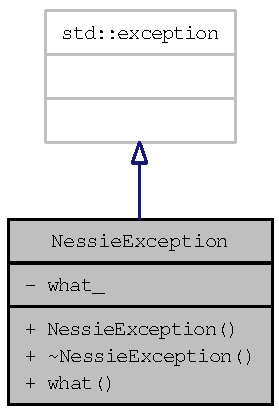
\includegraphics[width=85pt]{class_nessie_exception__inherit__graph}
\end{center}
\end{figure}
Collaboration diagram for NessieException:\nopagebreak
\begin{figure}[H]
\begin{center}
\leavevmode
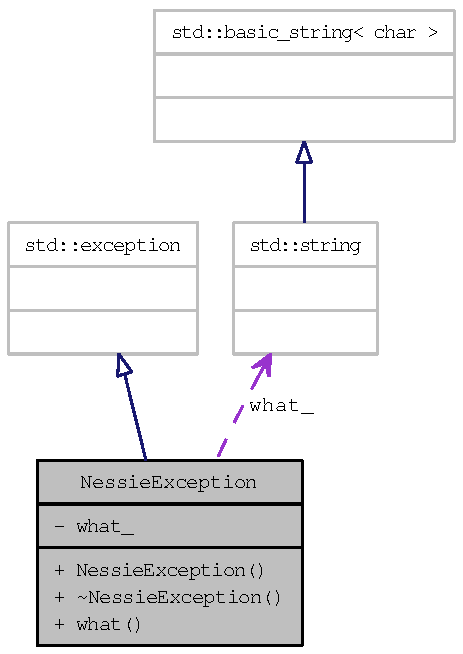
\includegraphics[width=129pt]{class_nessie_exception__coll__graph}
\end{center}
\end{figure}


\subsubsection{Detailed Description}
This class derives from std::exception class, so that all the exceptions either from this library or the STL itself can be caught using a reference to an 'exception' object.

\begin{Desc}
\item[Author:]Eliezer Talón (\href{mailto:elitalon@gmail.com}{\tt elitalon@gmail.com}) \end{Desc}
\begin{Desc}
\item[Date:]2008-10-03 \end{Desc}
\subsubsection*{Public Member Functions}
\begin{CompactItemize}
\item 
\hyperlink{class_nessie_exception_80c86c892438045635bf6a99da17e859}{NessieException} (const std::string \&what)
\begin{CompactList}\small\item\em Constructor. \item\end{CompactList}\item 
virtual \hyperlink{class_nessie_exception_19f44d2725dd53e2f10505a88e5773f2}{$\sim$NessieException} ()  throw ()
\begin{CompactList}\small\item\em Destructor. \item\end{CompactList}\item 
virtual const char $\ast$ \hyperlink{class_nessie_exception_a522c2ea164e88be0b26670170b33909}{what} () const   throw ()
\begin{CompactList}\small\item\em Returns a message that explains the exception raised. \item\end{CompactList}\end{CompactItemize}
\subsubsection*{Private Attributes}
\begin{CompactItemize}
\item 
\hypertarget{class_nessie_exception_3464c36d30d9baabd0b10ac4797d4b5b}{
std::string \hyperlink{class_nessie_exception_3464c36d30d9baabd0b10ac4797d4b5b}{what\_\-}}
\label{class_nessie_exception_3464c36d30d9baabd0b10ac4797d4b5b}

\begin{CompactList}\small\item\em Message that explains the exception raised. \item\end{CompactList}\end{CompactItemize}


\subsubsection{Constructor \& Destructor Documentation}
\hypertarget{class_nessie_exception_80c86c892438045635bf6a99da17e859}{
\index{NessieException@{NessieException}!NessieException@{NessieException}}
\index{NessieException@{NessieException}!NessieException@{NessieException}}
\paragraph[NessieException]{\setlength{\rightskip}{0pt plus 5cm}NessieException::NessieException (const std::string \& {\em what})}\hfill}
\label{class_nessie_exception_80c86c892438045635bf6a99da17e859}


\begin{Desc}
\item[Parameters:]
\begin{description}
\item[{\em what}]A message that explains the exception raised.\end{description}
\end{Desc}
\begin{Desc}
\item[Author:]Eliezer Talón (\href{mailto:elitalon@gmail.com}{\tt elitalon@gmail.com}) \end{Desc}
\begin{Desc}
\item[Date:]2008-10-03\end{Desc}
Initializes a \hyperlink{class_nessie_exception}{NessieException} object with a message. \hypertarget{class_nessie_exception_19f44d2725dd53e2f10505a88e5773f2}{
\index{NessieException@{NessieException}!$\sim$NessieException@{$\sim$NessieException}}
\index{$\sim$NessieException@{$\sim$NessieException}!NessieException@{NessieException}}
\paragraph[$\sim$NessieException]{\setlength{\rightskip}{0pt plus 5cm}NessieException::$\sim$NessieException ()  throw ()\hspace{0.3cm}{\tt  \mbox{[}virtual\mbox{]}}}\hfill}
\label{class_nessie_exception_19f44d2725dd53e2f10505a88e5773f2}


\begin{Desc}
\item[Author:]Eliezer Talón (\href{mailto:elitalon@gmail.com}{\tt elitalon@gmail.com}) \end{Desc}
\begin{Desc}
\item[Date:]2008-10-03\end{Desc}
Destroys a \hyperlink{class_nessie_exception}{NessieException} object. 

\subsubsection{Member Function Documentation}
\hypertarget{class_nessie_exception_a522c2ea164e88be0b26670170b33909}{
\index{NessieException@{NessieException}!what@{what}}
\index{what@{what}!NessieException@{NessieException}}
\paragraph[what]{\setlength{\rightskip}{0pt plus 5cm}const char $\ast$ NessieException::what () const  throw ()\hspace{0.3cm}{\tt  \mbox{[}virtual\mbox{]}}}\hfill}
\label{class_nessie_exception_a522c2ea164e88be0b26670170b33909}


\begin{Desc}
\item[Returns:]Message that explains the situation that caused the exception.\end{Desc}
\begin{Desc}
\item[Author:]Eliezer Talón (\href{mailto:elitalon@gmail.com}{\tt elitalon@gmail.com}) \end{Desc}
\begin{Desc}
\item[Date:]2008-10-03\end{Desc}
This method overrides the one in class std::exception. 

References what\_\-.
\hypertarget{class_pixel}{
\section{Pixel Class Reference}
\label{class_pixel}\index{Pixel@{Pixel}}
}
{\tt \#include $<$Pixel.h$>$}

Collaboration diagram for Pixel:\nopagebreak
\begin{figure}[H]
\begin{center}
\leavevmode
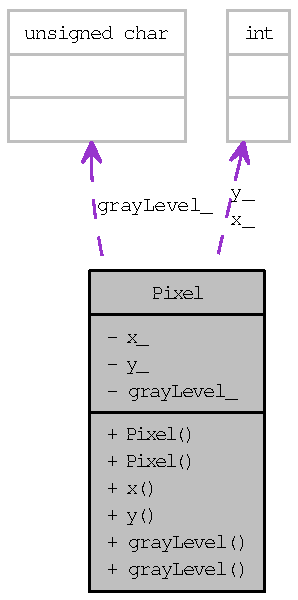
\includegraphics[width=89pt]{class_pixel__coll__graph}
\end{center}
\end{figure}


\subsection{Detailed Description}
Information about an image pixel. 

This class stores all the information of a pixel within a press clip. Every pixel has a location given by a pair of coordinates (x,y) and a color information in a grayscale colorspace of 256 levels.

The gray level of a pixel is a value between 0 and 255, where 0 corresponds to black and 255 corresponds to white. A monochromatic colorspace can be emulated using only 0 and 255.

\begin{Desc}
\item[Author:]Eliezer Talón (\href{mailto:elitalon@gmail.com}{\tt elitalon@gmail.com}) \end{Desc}
\begin{Desc}
\item[Date:]2008-10-10 \end{Desc}


Definition at line 22 of file Pixel.h.\subsection*{Public Member Functions}
\begin{CompactItemize}
\item 
\hyperlink{class_pixel_27ad99a2f705e635c42d242d530d4756}{Pixel} ()
\begin{CompactList}\small\item\em Constructor. \item\end{CompactList}\item 
\hyperlink{class_pixel_31103b6b7b52712789d1fdab7ab7ce29}{Pixel} (const unsigned int \&x, const unsigned int \&y, const unsigned char \&grayLevel)
\begin{CompactList}\small\item\em Constructor. \item\end{CompactList}\item 
unsigned int \hyperlink{class_pixel_68dafccc4588fb33d445641c2766316b}{x} () const 
\begin{CompactList}\small\item\em Returns the x coordinate of the pixel. \item\end{CompactList}\item 
unsigned int \hyperlink{class_pixel_204cc91a99e1e4f1d96c9cf6caf5747a}{y} () const 
\begin{CompactList}\small\item\em Returns the y coordinate of the pixel. \item\end{CompactList}\item 
unsigned char \hyperlink{class_pixel_d82be37dbb53c7ba48c5464b3a3382c6}{grayLevel} () const 
\begin{CompactList}\small\item\em Returns the pixel's gray level. \item\end{CompactList}\item 
void \hyperlink{class_pixel_d00a337e0d9765daafe3017f2d819df8}{grayLevel} (const unsigned char \&grayLevel)
\begin{CompactList}\small\item\em Sets the pixel's gray level. \item\end{CompactList}\end{CompactItemize}
\subsection*{Private Attributes}
\begin{CompactItemize}
\item 
\hypertarget{class_pixel_9f8a45ad3cbcab59543e4f7d4842ae6d}{
unsigned int \hyperlink{class_pixel_9f8a45ad3cbcab59543e4f7d4842ae6d}{x\_\-}}
\label{class_pixel_9f8a45ad3cbcab59543e4f7d4842ae6d}

\begin{CompactList}\small\item\em Pixel's X coordinate. \item\end{CompactList}\item 
\hypertarget{class_pixel_da45113dcf9ef4a0c3d5052db42da355}{
unsigned int \hyperlink{class_pixel_da45113dcf9ef4a0c3d5052db42da355}{y\_\-}}
\label{class_pixel_da45113dcf9ef4a0c3d5052db42da355}

\begin{CompactList}\small\item\em Pixel's Y coordinate. \item\end{CompactList}\item 
\hypertarget{class_pixel_e66fe85e02a9fe41e01ee520b87642e0}{
unsigned char \hyperlink{class_pixel_e66fe85e02a9fe41e01ee520b87642e0}{grayLevel\_\-}}
\label{class_pixel_e66fe85e02a9fe41e01ee520b87642e0}

\begin{CompactList}\small\item\em Pixel's gray level. \item\end{CompactList}\end{CompactItemize}


\subsection{Constructor \& Destructor Documentation}
\hypertarget{class_pixel_27ad99a2f705e635c42d242d530d4756}{
\index{Pixel@{Pixel}!Pixel@{Pixel}}
\index{Pixel@{Pixel}!Pixel@{Pixel}}
\subsubsection[Pixel]{\setlength{\rightskip}{0pt plus 5cm}Pixel::Pixel ()}}
\label{class_pixel_27ad99a2f705e635c42d242d530d4756}


Constructor. 

\begin{Desc}
\item[Author:]Eliezer Talón (\href{mailto:elitalon@gmail.com}{\tt elitalon@gmail.com}) \end{Desc}
\begin{Desc}
\item[Date:]2008-10-10\end{Desc}
Initializes a empty \hyperlink{class_pixel}{Pixel} object located at (0,0) 

Definition at line 12 of file Pixel.cpp.\hypertarget{class_pixel_31103b6b7b52712789d1fdab7ab7ce29}{
\index{Pixel@{Pixel}!Pixel@{Pixel}}
\index{Pixel@{Pixel}!Pixel@{Pixel}}
\subsubsection[Pixel]{\setlength{\rightskip}{0pt plus 5cm}Pixel::Pixel (const unsigned int \& {\em x}, \/  const unsigned int \& {\em y}, \/  const unsigned char \& {\em grayLevel})}}
\label{class_pixel_31103b6b7b52712789d1fdab7ab7ce29}


Constructor. 

\begin{Desc}
\item[Parameters:]
\begin{description}
\item[{\em x}]X coordinate (row) of the pixel \item[{\em y}]Y coordinate (colum) of the pixel \item[{\em grayLevel}]\hyperlink{class_pixel}{Pixel} gray level\end{description}
\end{Desc}
\begin{Desc}
\item[Author:]Eliezer Talón (\href{mailto:elitalon@gmail.com}{\tt elitalon@gmail.com}) \end{Desc}
\begin{Desc}
\item[Date:]2008-10-10\end{Desc}
Initializes a \hyperlink{class_pixel}{Pixel} object with the coordinates and gray level provided. If the gray level 

Definition at line 22 of file Pixel.cpp.

\subsection{Member Function Documentation}
\hypertarget{class_pixel_68dafccc4588fb33d445641c2766316b}{
\index{Pixel@{Pixel}!x@{x}}
\index{x@{x}!Pixel@{Pixel}}
\subsubsection[x]{\setlength{\rightskip}{0pt plus 5cm}unsigned int Pixel::x () const\hspace{0.3cm}{\tt  \mbox{[}inline\mbox{]}}}}
\label{class_pixel_68dafccc4588fb33d445641c2766316b}


Returns the x coordinate of the pixel. 

\begin{Desc}
\item[Returns:]The x coordinate (row) of the pixel\end{Desc}
\begin{Desc}
\item[Author:]Eliezer Talón (\href{mailto:elitalon@gmail.com}{\tt elitalon@gmail.com}) \end{Desc}
\begin{Desc}
\item[Date:]2008-10-08 \end{Desc}


Definition at line 118 of file Pixel.h.\hypertarget{class_pixel_204cc91a99e1e4f1d96c9cf6caf5747a}{
\index{Pixel@{Pixel}!y@{y}}
\index{y@{y}!Pixel@{Pixel}}
\subsubsection[y]{\setlength{\rightskip}{0pt plus 5cm}unsigned int Pixel::y () const\hspace{0.3cm}{\tt  \mbox{[}inline\mbox{]}}}}
\label{class_pixel_204cc91a99e1e4f1d96c9cf6caf5747a}


Returns the y coordinate of the pixel. 

\begin{Desc}
\item[Returns:]The y coordinate (column) of the pixel\end{Desc}
\begin{Desc}
\item[Author:]Eliezer Talón (\href{mailto:elitalon@gmail.com}{\tt elitalon@gmail.com}) \end{Desc}
\begin{Desc}
\item[Date:]2008-10-08 \end{Desc}


Definition at line 127 of file Pixel.h.\hypertarget{class_pixel_d82be37dbb53c7ba48c5464b3a3382c6}{
\index{Pixel@{Pixel}!grayLevel@{grayLevel}}
\index{grayLevel@{grayLevel}!Pixel@{Pixel}}
\subsubsection[grayLevel]{\setlength{\rightskip}{0pt plus 5cm}unsigned char Pixel::grayLevel () const\hspace{0.3cm}{\tt  \mbox{[}inline\mbox{]}}}}
\label{class_pixel_d82be37dbb53c7ba48c5464b3a3382c6}


Returns the pixel's gray level. 

\begin{Desc}
\item[Returns:]The gray level of the pixel\end{Desc}
\begin{Desc}
\item[Author:]Eliezer Talón (\href{mailto:elitalon@gmail.com}{\tt elitalon@gmail.com}) \end{Desc}
\begin{Desc}
\item[Date:]2008-09-26 \end{Desc}


Definition at line 137 of file Pixel.h.\hypertarget{class_pixel_d00a337e0d9765daafe3017f2d819df8}{
\index{Pixel@{Pixel}!grayLevel@{grayLevel}}
\index{grayLevel@{grayLevel}!Pixel@{Pixel}}
\subsubsection[grayLevel]{\setlength{\rightskip}{0pt plus 5cm}void Pixel::grayLevel (const unsigned char \& {\em grayLevel})\hspace{0.3cm}{\tt  \mbox{[}inline\mbox{]}}}}
\label{class_pixel_d00a337e0d9765daafe3017f2d819df8}


Sets the pixel's gray level. 

\begin{Desc}
\item[Parameters:]
\begin{description}
\item[{\em grayLevel}]The gray level of the pixel\end{description}
\end{Desc}
\begin{Desc}
\item[Author:]Eliezer Talón (\href{mailto:elitalon@gmail.com}{\tt elitalon@gmail.com}) \end{Desc}
\begin{Desc}
\item[Date:]2008-10-10 \end{Desc}


Definition at line 146 of file Pixel.h.

The documentation for this class was generated from the following files:\begin{CompactItemize}
\item 
\hyperlink{_pixel_8h}{Pixel.h (132)}\item 
\hyperlink{_pixel_8cpp}{Pixel.cpp (132)}\end{CompactItemize}

\hypertarget{class_preprocessor}{
\section{Preprocessor Class Reference}
\label{class_preprocessor}\index{Preprocessor@{Preprocessor}}
}
{\tt \#include $<$Preprocessor.h$>$}

Collaboration diagram for Preprocessor:\nopagebreak
\begin{figure}[H]
\begin{center}
\leavevmode
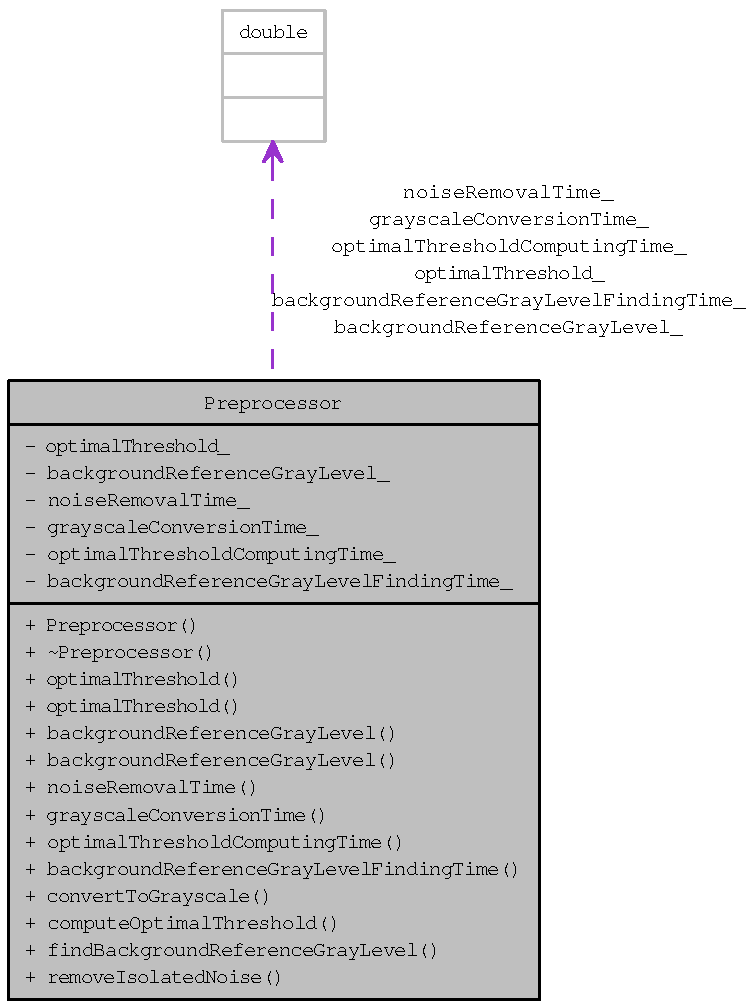
\includegraphics[width=400pt]{class_preprocessor__coll__graph}
\end{center}
\end{figure}


\subsection{Detailed Description}
\hyperlink{class_preprocessor}{Preprocessor} of the OCR process. 

This class encapsulates all the methods related to preprocessing stage. Its task is to enhance the image quality by applying some techniques of image preprocessing theory and compute a number of parameters such as the optimal thresolding value or the background reference gray level

\begin{Desc}
\item[See also:]\hyperlink{class_clip}{Clip}\end{Desc}
\begin{Desc}
\item[Author:]Eliezer Talón (\href{mailto:elitalon@gmail.com}{\tt elitalon@gmail.com}) \end{Desc}
\begin{Desc}
\item[Date:]2008-10-11 \end{Desc}


Definition at line 25 of file Preprocessor.h.\subsection*{Public Member Functions}
\begin{CompactItemize}
\item 
\hyperlink{class_preprocessor_da966c8b83e7c3bcd8759549c3cdf688}{Preprocessor} ()
\begin{CompactList}\small\item\em Constructor. \item\end{CompactList}\item 
unsigned char \hyperlink{class_preprocessor_1d8eaa1cf786941dbfa1eca95b46ce0c}{optimalThreshold} () const 
\begin{CompactList}\small\item\em Returns the optimal threshold found in the last clip used. \item\end{CompactList}\item 
void \hyperlink{class_preprocessor_1fc44d7d19944f3c3addd3a576c37414}{optimalThreshold} (const unsigned char \&threshold)
\begin{CompactList}\small\item\em Sets the optimal threshold to use in algorithms. \item\end{CompactList}\item 
unsigned char \hyperlink{class_preprocessor_9a2684181b5f43051fe53d7d2950dd36}{backgroundReferenceGrayLevel} () const 
\begin{CompactList}\small\item\em Returns the background reference gray level in the last clip used. \item\end{CompactList}\item 
double \hyperlink{class_preprocessor_0cccd23820430541f18f2b24dbfd0784}{noiseRemovalTime} () const 
\begin{CompactList}\small\item\em Returns the elapsed time while applying the 'isolated noise removal' algorithm. \item\end{CompactList}\item 
double \hyperlink{class_preprocessor_72dd29238c4202698e67dcb26a47f4b5}{optimalThresholdComputingTime} () const 
\begin{CompactList}\small\item\em Returns the elapsed time while founding the optimal threshold within the clip. \item\end{CompactList}\item 
double \hyperlink{class_preprocessor_3189cad5515476d54cc14effcf983fc7}{backgroundReferenceGrayLevelFindingTime} () const 
\begin{CompactList}\small\item\em Returns the elapsed time while computing the background reference gray level within the clip. \item\end{CompactList}\item 
unsigned char \hyperlink{class_preprocessor_0e146cafa6b8b31f4f4ed189a970db7a}{computeOptimalThreshold} (const \hyperlink{class_clip}{Clip} \&clip)
\begin{CompactList}\small\item\em Computes the optimal threshold value within a clip. \item\end{CompactList}\item 
unsigned char \hyperlink{class_preprocessor_19aa90451cf6f99854833c05d3e71270}{findBackgroundReferenceGrayLevel} (const \hyperlink{class_clip}{Clip} \&clip, const unsigned int \&referenceGrayLevelNeighbours=4)
\begin{CompactList}\small\item\em Computes the background reference gray level value within a clip. \item\end{CompactList}\item 
void \hyperlink{class_preprocessor_a365f69af48cae608071e9943f300dd5}{removeIsolatedNoise} (\hyperlink{class_clip}{Clip} \&clip, const unsigned int \&isolationCoefficient=1)
\begin{CompactList}\small\item\em Applies the 'isolated noise removal' algorithm. \item\end{CompactList}\end{CompactItemize}
\subsection*{Private Attributes}
\begin{CompactItemize}
\item 
\hypertarget{class_preprocessor_865b1e28dd9535b96f70727a550104fe}{
unsigned char \hyperlink{class_preprocessor_865b1e28dd9535b96f70727a550104fe}{optimalThreshold\_\-}}
\label{class_preprocessor_865b1e28dd9535b96f70727a550104fe}

\begin{CompactList}\small\item\em Optimal threshold value within the clip. \item\end{CompactList}\item 
\hypertarget{class_preprocessor_2c9e44ff6522b2ce35d6bc6161ad2680}{
unsigned char \hyperlink{class_preprocessor_2c9e44ff6522b2ce35d6bc6161ad2680}{backgroundReferenceGrayLevel\_\-}}
\label{class_preprocessor_2c9e44ff6522b2ce35d6bc6161ad2680}

\begin{CompactList}\small\item\em Background reference gray level. \item\end{CompactList}\item 
\hypertarget{class_preprocessor_386a5118bd982b2377c1fc5d67ebb7ac}{
double \hyperlink{class_preprocessor_386a5118bd982b2377c1fc5d67ebb7ac}{noiseRemovalTime\_\-}}
\label{class_preprocessor_386a5118bd982b2377c1fc5d67ebb7ac}

\begin{CompactList}\small\item\em Elapsed time when applying the 'isolated noise removal' algorithm. \item\end{CompactList}\item 
\hypertarget{class_preprocessor_d606fe1f0be7f7be60583f59278e2df6}{
double \hyperlink{class_preprocessor_d606fe1f0be7f7be60583f59278e2df6}{optimalThresholdComputingTime\_\-}}
\label{class_preprocessor_d606fe1f0be7f7be60583f59278e2df6}

\begin{CompactList}\small\item\em Elapsed time when converting the image to a grayscale colorspace. \item\end{CompactList}\item 
\hypertarget{class_preprocessor_140ea3fa7bbd4e8fef54912d65c4e926}{
double \hyperlink{class_preprocessor_140ea3fa7bbd4e8fef54912d65c4e926}{backgroundReferenceGrayLevelFindingTime\_\-}}
\label{class_preprocessor_140ea3fa7bbd4e8fef54912d65c4e926}

\begin{CompactList}\small\item\em Elapsed time when computing the background gray level. \item\end{CompactList}\end{CompactItemize}


\subsection{Constructor \& Destructor Documentation}
\hypertarget{class_preprocessor_da966c8b83e7c3bcd8759549c3cdf688}{
\index{Preprocessor@{Preprocessor}!Preprocessor@{Preprocessor}}
\index{Preprocessor@{Preprocessor}!Preprocessor@{Preprocessor}}
\subsubsection[Preprocessor]{\setlength{\rightskip}{0pt plus 5cm}Preprocessor::Preprocessor ()}}
\label{class_preprocessor_da966c8b83e7c3bcd8759549c3cdf688}


Constructor. 

\begin{Desc}
\item[Author:]Eliezer Talón (\href{mailto:elitalon@gmail.com}{\tt elitalon@gmail.com}) \end{Desc}
\begin{Desc}
\item[Date:]2008-10-08\end{Desc}
Initializes a \hyperlink{class_preprocessor}{Preprocessor} object 

Definition at line 20 of file Preprocessor.cpp.

\subsection{Member Function Documentation}
\hypertarget{class_preprocessor_1d8eaa1cf786941dbfa1eca95b46ce0c}{
\index{Preprocessor@{Preprocessor}!optimalThreshold@{optimalThreshold}}
\index{optimalThreshold@{optimalThreshold}!Preprocessor@{Preprocessor}}
\subsubsection[optimalThreshold]{\setlength{\rightskip}{0pt plus 5cm}unsigned char Preprocessor::optimalThreshold () const\hspace{0.3cm}{\tt  \mbox{[}inline\mbox{]}}}}
\label{class_preprocessor_1d8eaa1cf786941dbfa1eca95b46ce0c}


Returns the optimal threshold found in the last clip used. 

\begin{Desc}
\item[Returns:]Current optimal threshold computed from the last clip used\end{Desc}
\begin{Desc}
\item[Author:]Eliezer Talón (\href{mailto:elitalon@gmail.com}{\tt elitalon@gmail.com}) \end{Desc}
\begin{Desc}
\item[Date:]2008-10-08 \end{Desc}


Definition at line 184 of file Preprocessor.h.\hypertarget{class_preprocessor_1fc44d7d19944f3c3addd3a576c37414}{
\index{Preprocessor@{Preprocessor}!optimalThreshold@{optimalThreshold}}
\index{optimalThreshold@{optimalThreshold}!Preprocessor@{Preprocessor}}
\subsubsection[optimalThreshold]{\setlength{\rightskip}{0pt plus 5cm}void Preprocessor::optimalThreshold (const unsigned char \& {\em threshold})\hspace{0.3cm}{\tt  \mbox{[}inline\mbox{]}}}}
\label{class_preprocessor_1fc44d7d19944f3c3addd3a576c37414}


Sets the optimal threshold to use in algorithms. 

\begin{Desc}
\item[Parameters:]
\begin{description}
\item[{\em threshold}]A value between 0 and 255 that stablishes the optimal threshold of a clip\end{description}
\end{Desc}
\begin{Desc}
\item[Author:]Eliezer Talón (\href{mailto:elitalon@gmail.com}{\tt elitalon@gmail.com}) \end{Desc}
\begin{Desc}
\item[Date:]2008-10-08 \end{Desc}


Definition at line 193 of file Preprocessor.h.\hypertarget{class_preprocessor_9a2684181b5f43051fe53d7d2950dd36}{
\index{Preprocessor@{Preprocessor}!backgroundReferenceGrayLevel@{backgroundReferenceGrayLevel}}
\index{backgroundReferenceGrayLevel@{backgroundReferenceGrayLevel}!Preprocessor@{Preprocessor}}
\subsubsection[backgroundReferenceGrayLevel]{\setlength{\rightskip}{0pt plus 5cm}unsigned char Preprocessor::backgroundReferenceGrayLevel () const\hspace{0.3cm}{\tt  \mbox{[}inline\mbox{]}}}}
\label{class_preprocessor_9a2684181b5f43051fe53d7d2950dd36}


Returns the background reference gray level in the last clip used. 

\begin{Desc}
\item[Returns:]Reference background gray level in the last clip used\end{Desc}
\begin{Desc}
\item[Author:]Eliezer Talón (\href{mailto:elitalon@gmail.com}{\tt elitalon@gmail.com}) \end{Desc}
\begin{Desc}
\item[Date:]2008-10-08 \end{Desc}


Definition at line 202 of file Preprocessor.h.\hypertarget{class_preprocessor_0cccd23820430541f18f2b24dbfd0784}{
\index{Preprocessor@{Preprocessor}!noiseRemovalTime@{noiseRemovalTime}}
\index{noiseRemovalTime@{noiseRemovalTime}!Preprocessor@{Preprocessor}}
\subsubsection[noiseRemovalTime]{\setlength{\rightskip}{0pt plus 5cm}double Preprocessor::noiseRemovalTime () const\hspace{0.3cm}{\tt  \mbox{[}inline\mbox{]}}}}
\label{class_preprocessor_0cccd23820430541f18f2b24dbfd0784}


Returns the elapsed time while applying the 'isolated noise removal' algorithm. 

\begin{Desc}
\item[Returns:]Elapsed time when applying the 'isolated noise removal' algorithm\end{Desc}
\begin{Desc}
\item[Author:]Eliezer Talón (\href{mailto:elitalon@gmail.com}{\tt elitalon@gmail.com}) \end{Desc}
\begin{Desc}
\item[Date:]2008-10-08 \end{Desc}


Definition at line 211 of file Preprocessor.h.

Referenced by Recognizer::obtainText().\hypertarget{class_preprocessor_72dd29238c4202698e67dcb26a47f4b5}{
\index{Preprocessor@{Preprocessor}!optimalThresholdComputingTime@{optimalThresholdComputingTime}}
\index{optimalThresholdComputingTime@{optimalThresholdComputingTime}!Preprocessor@{Preprocessor}}
\subsubsection[optimalThresholdComputingTime]{\setlength{\rightskip}{0pt plus 5cm}double Preprocessor::optimalThresholdComputingTime () const\hspace{0.3cm}{\tt  \mbox{[}inline\mbox{]}}}}
\label{class_preprocessor_72dd29238c4202698e67dcb26a47f4b5}


Returns the elapsed time while founding the optimal threshold within the clip. 

\begin{Desc}
\item[Returns:]Elapsed time while founding the optimal threshold within the clip\end{Desc}
\begin{Desc}
\item[Author:]Eliezer Talón (\href{mailto:elitalon@gmail.com}{\tt elitalon@gmail.com}) \end{Desc}
\begin{Desc}
\item[Date:]2008-10-08 \end{Desc}


Definition at line 220 of file Preprocessor.h.

Referenced by Recognizer::obtainText().\hypertarget{class_preprocessor_3189cad5515476d54cc14effcf983fc7}{
\index{Preprocessor@{Preprocessor}!backgroundReferenceGrayLevelFindingTime@{backgroundReferenceGrayLevelFindingTime}}
\index{backgroundReferenceGrayLevelFindingTime@{backgroundReferenceGrayLevelFindingTime}!Preprocessor@{Preprocessor}}
\subsubsection[backgroundReferenceGrayLevelFindingTime]{\setlength{\rightskip}{0pt plus 5cm}double Preprocessor::backgroundReferenceGrayLevelFindingTime () const\hspace{0.3cm}{\tt  \mbox{[}inline\mbox{]}}}}
\label{class_preprocessor_3189cad5515476d54cc14effcf983fc7}


Returns the elapsed time while computing the background reference gray level within the clip. 

\begin{Desc}
\item[Returns:]Elapsed time while computing the background reference gray level\end{Desc}
\begin{Desc}
\item[Author:]Eliezer Talón (\href{mailto:elitalon@gmail.com}{\tt elitalon@gmail.com}) \end{Desc}
\begin{Desc}
\item[Date:]2008-10-08 \end{Desc}


Definition at line 229 of file Preprocessor.h.

Referenced by Recognizer::obtainText().\hypertarget{class_preprocessor_0e146cafa6b8b31f4f4ed189a970db7a}{
\index{Preprocessor@{Preprocessor}!computeOptimalThreshold@{computeOptimalThreshold}}
\index{computeOptimalThreshold@{computeOptimalThreshold}!Preprocessor@{Preprocessor}}
\subsubsection[computeOptimalThreshold]{\setlength{\rightskip}{0pt plus 5cm}unsigned char Preprocessor::computeOptimalThreshold (const {\bf Clip} \& {\em clip})}}
\label{class_preprocessor_0e146cafa6b8b31f4f4ed189a970db7a}


Computes the optimal threshold value within a clip. 

\begin{Desc}
\item[Precondition:]You MUST call \hyperlink{class_preprocessor_19aa90451cf6f99854833c05d3e71270}{findBackgroundReferenceGrayLevel()} method before calling this one, since it sets internal attributes.\end{Desc}
\begin{Desc}
\item[Parameters:]
\begin{description}
\item[{\em clip}]The clip where applying the algorithm over\end{description}
\end{Desc}
\begin{Desc}
\item[Returns:]The optimal threshold of the clip\end{Desc}
\begin{Desc}
\item[Author:]Eliezer Talón (\href{mailto:elitalon@gmail.com}{\tt elitalon@gmail.com}) \end{Desc}
\begin{Desc}
\item[Date:]2008-10-11\end{Desc}
To compute the optimal threshold we follow the strategy proposed by Sonka M., Hlavac V. and Boyle R. in \char`\"{}Image Processing, Analysis and Machine Vision\char`\"{} (Thomson Learning, 2008). The target is to find a mean value between the mean value of background's gray level and the mean value of objects' gray level, starting from an initial threshold value. 

Definition at line 33 of file Preprocessor.cpp.

Referenced by Recognizer::obtainText().\hypertarget{class_preprocessor_19aa90451cf6f99854833c05d3e71270}{
\index{Preprocessor@{Preprocessor}!findBackgroundReferenceGrayLevel@{findBackgroundReferenceGrayLevel}}
\index{findBackgroundReferenceGrayLevel@{findBackgroundReferenceGrayLevel}!Preprocessor@{Preprocessor}}
\subsubsection[findBackgroundReferenceGrayLevel]{\setlength{\rightskip}{0pt plus 5cm}unsigned char Preprocessor::findBackgroundReferenceGrayLevel (const {\bf Clip} \& {\em clip}, \/  const unsigned int \& {\em referenceGrayLevelNeighbours} = {\tt 4})}}
\label{class_preprocessor_19aa90451cf6f99854833c05d3e71270}


Computes the background reference gray level value within a clip. 

\begin{Desc}
\item[Parameters:]
\begin{description}
\item[{\em clip}]The clip where applying the algorithm over \item[{\em referenceGrayLevelNeighbours}]Number of neighbours of the more frequent gray level to explore on each direction\end{description}
\end{Desc}
\begin{Desc}
\item[Returns:]The reference gray level of the background\end{Desc}
\begin{Desc}
\item[Author:]Eliezer Talón (\href{mailto:elitalon@gmail.com}{\tt elitalon@gmail.com}) \end{Desc}
\begin{Desc}
\item[Date:]2008-10-11\end{Desc}
To find the reference gray level of the background it is assumed that there are more pixels belonging to the background than belonging to the foreground. Then, we search the more frequent gray level and its neighbours. Finally, we compute a gray level weighted mean using all those values. 

Definition at line 91 of file Preprocessor.cpp.

Referenced by Recognizer::obtainText().\hypertarget{class_preprocessor_a365f69af48cae608071e9943f300dd5}{
\index{Preprocessor@{Preprocessor}!removeIsolatedNoise@{removeIsolatedNoise}}
\index{removeIsolatedNoise@{removeIsolatedNoise}!Preprocessor@{Preprocessor}}
\subsubsection[removeIsolatedNoise]{\setlength{\rightskip}{0pt plus 5cm}void Preprocessor::removeIsolatedNoise ({\bf Clip} \& {\em clip}, \/  const unsigned int \& {\em isolationCoefficient} = {\tt 1})}}
\label{class_preprocessor_a365f69af48cae608071e9943f300dd5}


Applies the 'isolated noise removal' algorithm. 

\begin{Desc}
\item[Precondition:]You MUST call \hyperlink{class_preprocessor_0e146cafa6b8b31f4f4ed189a970db7a}{computeOptimalThreshold()} and \hyperlink{class_preprocessor_19aa90451cf6f99854833c05d3e71270}{findBackgroundReferenceGrayLevel()} methods before calling this one, since they set internal attributes.\end{Desc}
\begin{Desc}
\item[Parameters:]
\begin{description}
\item[\mbox{$\leftrightarrow$} {\em clip}]The clip where applying the algorithm over \item[{\em isolationCoefficient}]The maximum noisy neighbours for a pixel to consider it as isolated\end{description}
\end{Desc}
\begin{Desc}
\item[Author:]Eliezer Talón (\href{mailto:elitalon@gmail.com}{\tt elitalon@gmail.com}) \end{Desc}
\begin{Desc}
\item[Date:]2008-10-11\end{Desc}
The 'isolated noise removal' algorithm tries to eliminate isolated noisy pixels from an clip. The isolationCoefficient parameter defines how much isolated should be a noisy pixel to be removed. That means a noisy pixel will be removed whenever it has as much neighbours whose gray level is over a threshold value as isolationCoefficient. 

Definition at line 163 of file Preprocessor.cpp.

Referenced by Recognizer::obtainText().

The documentation for this class was generated from the following files:\begin{CompactItemize}
\item 
\hyperlink{_preprocessor_8h}{Preprocessor.h (138)}\item 
\hyperlink{_preprocessor_8cpp}{Preprocessor.cpp (138)}\end{CompactItemize}

\hypertarget{class_statistics}{
\section{Statistics Class Reference}
\label{class_statistics}\index{Statistics@{Statistics}}
}
{\tt \#include $<$Statistics.hpp$>$}

Collaboration diagram for Statistics:\nopagebreak
\begin{figure}[H]
\begin{center}
\leavevmode
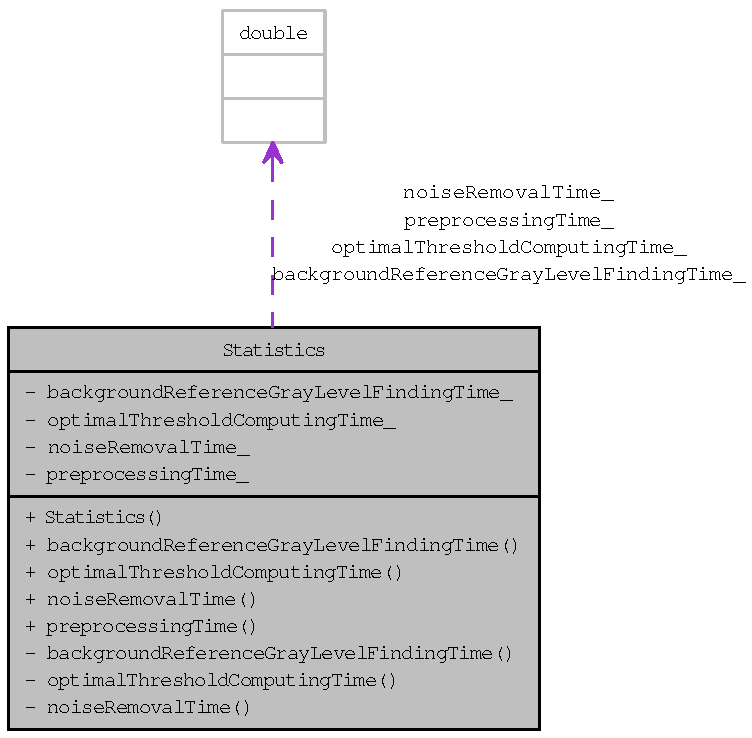
\includegraphics[height=400pt]{class_statistics__coll__graph}
\end{center}
\end{figure}


\subsection{Detailed Description}
\hyperlink{class_statistics}{Statistics} about the text recognition process. 

This class stores a number of statistical data regarding the elapsed time during the text recognition process, accumulated internally mostly in algorithms.

\begin{Desc}
\item[Author:]Eliezer Talón (\href{mailto:elitalon@gmail.com}{\tt elitalon@gmail.com}) \end{Desc}
\begin{Desc}
\item[Date:]2008-10-08 \end{Desc}


Definition at line 19 of file Statistics.hpp.\subsection*{Public Member Functions}
\begin{CompactItemize}
\item 
\hyperlink{class_statistics_60ddd90a571ed4c3ce8c0f6317a36d63}{Statistics} ()
\begin{CompactList}\small\item\em Constructor. \item\end{CompactList}\item 
\hyperlink{class_statistics}{Statistics} \hyperlink{class_statistics_cb07c98a63e07fdb1476ffb282b84676}{operator+} (const \hyperlink{class_statistics}{Statistics} \&statistics) const 
\begin{CompactList}\small\item\em Allows the sum of two different statistics. \item\end{CompactList}\item 
\hyperlink{class_statistics}{Statistics} \hyperlink{class_statistics_529bed34d909d88440214d6983779043}{operator-} (const \hyperlink{class_statistics}{Statistics} \&statistics) const 
\begin{CompactList}\small\item\em Allows the subtraction of two different statistics. \item\end{CompactList}\item 
const double \& \hyperlink{class_statistics_d70a464a72d94c795097608e2a18550a}{backgroundReferenceGrayLevelFindingTime} () const 
\begin{CompactList}\small\item\em Returns the elapsed time in the reference gray level of the background finding algorithm. \item\end{CompactList}\item 
const double \& \hyperlink{class_statistics_87bdb5b4f7a88cb74d0072fd0c7a2248}{optimalThresholdComputingTime} () const 
\begin{CompactList}\small\item\em Returns the elapsed time in the optimal threshold computing algorithm. \item\end{CompactList}\item 
const double \& \hyperlink{class_statistics_ba44f1b2567a77f99ee15c11bda6312a}{noiseRemovalTime} () const 
\begin{CompactList}\small\item\em Returns the elapsed time in the noise removal algorithm. \item\end{CompactList}\item 
const double \& \hyperlink{class_statistics_9b1c2d1f1338069346c80293a2c11b6d}{preprocessingTime} () const 
\begin{CompactList}\small\item\em Returns the total elapsed time within the preprocessing stage. \item\end{CompactList}\item 
const double \& \hyperlink{class_statistics_51a8c70011a201873db8f388dad733ac}{thresholdingTime} () const 
\begin{CompactList}\small\item\em Returns the elapsed time while applying the thresholding algorithm. \item\end{CompactList}\item 
const double \& \hyperlink{class_statistics_9437fbc6726c6179b3ee4c130520e642}{shapesFindingTime} () const 
\begin{CompactList}\small\item\em Returns the elapsed time while finding the shapes in a clip. \item\end{CompactList}\item 
const double \& \hyperlink{class_statistics_f4c992e9970bce97b9a33100db689739}{segmentationTime} () const 
\begin{CompactList}\small\item\em Returns the total elapsed time within the segmentation stage. \item\end{CompactList}\end{CompactItemize}
\subsection*{Private Member Functions}
\begin{CompactItemize}
\item 
void \hyperlink{class_statistics_f8a60e8a89be8fe8b2c46782681c1a2c}{backgroundReferenceGrayLevelFindingTime} (const double \&time)
\begin{CompactList}\small\item\em Sets the elapsed time in the reference gray level of the background finding algorithm. \item\end{CompactList}\item 
void \hyperlink{class_statistics_eed35a930f29f4596f3715306e1e1dbc}{optimalThresholdComputingTime} (const double \&time)
\begin{CompactList}\small\item\em Sets the elapsed time in the optimal threshold computing algorithm. \item\end{CompactList}\item 
void \hyperlink{class_statistics_4ad24aec4e5491b7d3afca143e6deb05}{noiseRemovalTime} (const double \&time)
\begin{CompactList}\small\item\em Sets the elapsed time in the noise removal algorithm. \item\end{CompactList}\item 
void \hyperlink{class_statistics_ca6e07bda50783e324e8c51d8c815019}{thresholdingTime} (const double \&time)
\begin{CompactList}\small\item\em Sets the elapsed time in the thresholding algorithm. \item\end{CompactList}\item 
void \hyperlink{class_statistics_bc0a0e96adba6828ffb915a617b58ed2}{shapesFindingTime} (const double \&time)
\begin{CompactList}\small\item\em Sets the elapsed time in the shapes finding algorithm. \item\end{CompactList}\end{CompactItemize}
\subsection*{Private Attributes}
\begin{CompactItemize}
\item 
\hypertarget{class_statistics_ac1d32288eac323391e66b2ff1a878e8}{
double \hyperlink{class_statistics_ac1d32288eac323391e66b2ff1a878e8}{backgroundReferenceGrayLevelFindingTime\_\-}}
\label{class_statistics_ac1d32288eac323391e66b2ff1a878e8}

\begin{CompactList}\small\item\em Elapsed time in the reference gray level of the background finding algorithm. \item\end{CompactList}\item 
\hypertarget{class_statistics_b8cb0f26533cee29b94f3a556b00e943}{
double \hyperlink{class_statistics_b8cb0f26533cee29b94f3a556b00e943}{optimalThresholdComputingTime\_\-}}
\label{class_statistics_b8cb0f26533cee29b94f3a556b00e943}

\begin{CompactList}\small\item\em Elapsed time in the optimal threshold computing algorithm. \item\end{CompactList}\item 
\hypertarget{class_statistics_acacd5443d740dda6ddd83deb777ec4b}{
double \hyperlink{class_statistics_acacd5443d740dda6ddd83deb777ec4b}{noiseRemovalTime\_\-}}
\label{class_statistics_acacd5443d740dda6ddd83deb777ec4b}

\begin{CompactList}\small\item\em Elapsed time in the noise removal algorithm. \item\end{CompactList}\item 
\hypertarget{class_statistics_91e724d9ef7b96e1df3310c61234ebbd}{
double \hyperlink{class_statistics_91e724d9ef7b96e1df3310c61234ebbd}{preprocessingTime\_\-}}
\label{class_statistics_91e724d9ef7b96e1df3310c61234ebbd}

\begin{CompactList}\small\item\em Total elapsed time within the preprocessing stage. \item\end{CompactList}\item 
\hypertarget{class_statistics_e830ef1e50443eda784cadb18ca2b0d1}{
double \hyperlink{class_statistics_e830ef1e50443eda784cadb18ca2b0d1}{thresholdingTime\_\-}}
\label{class_statistics_e830ef1e50443eda784cadb18ca2b0d1}

\begin{CompactList}\small\item\em Elapsed time while applying the thresholding algorithm. \item\end{CompactList}\item 
\hypertarget{class_statistics_902172424d5011a89726319dfd32fa19}{
double \hyperlink{class_statistics_902172424d5011a89726319dfd32fa19}{shapesFindingTime\_\-}}
\label{class_statistics_902172424d5011a89726319dfd32fa19}

\begin{CompactList}\small\item\em Elapsed time while finding the shapes in a clip. \item\end{CompactList}\item 
\hypertarget{class_statistics_89ff84bd9b9b80585822c461ec25c8eb}{
double \hyperlink{class_statistics_89ff84bd9b9b80585822c461ec25c8eb}{segmentationTime\_\-}}
\label{class_statistics_89ff84bd9b9b80585822c461ec25c8eb}

\begin{CompactList}\small\item\em Total elapsed time within the segmentation stage. \item\end{CompactList}\end{CompactItemize}
\subsection*{Friends}
\begin{CompactItemize}
\item 
\hypertarget{class_statistics_11123fa51c07995419270030024a7dfe}{
class \hyperlink{class_statistics_11123fa51c07995419270030024a7dfe}{Recognizer}}
\label{class_statistics_11123fa51c07995419270030024a7dfe}

\begin{CompactList}\small\item\em Declares the class \hyperlink{class_recognizer}{Recognizer} as friend. \item\end{CompactList}\end{CompactItemize}


\subsection{Constructor \& Destructor Documentation}
\hypertarget{class_statistics_60ddd90a571ed4c3ce8c0f6317a36d63}{
\index{Statistics@{Statistics}!Statistics@{Statistics}}
\index{Statistics@{Statistics}!Statistics@{Statistics}}
\subsubsection[Statistics]{\setlength{\rightskip}{0pt plus 5cm}Statistics::Statistics ()}}
\label{class_statistics_60ddd90a571ed4c3ce8c0f6317a36d63}


Constructor. 

\begin{Desc}
\item[Author:]Eliezer Talón (\href{mailto:elitalon@gmail.com}{\tt elitalon@gmail.com}) \end{Desc}
\begin{Desc}
\item[Date:]2008-10-04\end{Desc}
Initializes a \hyperlink{class_statistics}{Statistics} object with timers set to 0.0 

Definition at line 12 of file Statistics.cpp.

\subsection{Member Function Documentation}
\hypertarget{class_statistics_cb07c98a63e07fdb1476ffb282b84676}{
\index{Statistics@{Statistics}!operator+@{operator+}}
\index{operator+@{operator+}!Statistics@{Statistics}}
\subsubsection[operator+]{\setlength{\rightskip}{0pt plus 5cm}{\bf Statistics} Statistics::operator+ (const {\bf Statistics} \& {\em statistics}) const\hspace{0.3cm}{\tt  \mbox{[}inline\mbox{]}}}}
\label{class_statistics_cb07c98a63e07fdb1476ffb282b84676}


Allows the sum of two different statistics. 

\begin{Desc}
\item[Parameters:]
\begin{description}
\item[{\em statistics}]A set of statistical data as the second operand\end{description}
\end{Desc}
\begin{Desc}
\item[Returns:]A new set of statistical data as a result of summing the time parameters of both objects each other\end{Desc}
\begin{Desc}
\item[Author:]Eliezer Talón (\href{mailto:elitalon@gmail.com}{\tt elitalon@gmail.com}) \end{Desc}
\begin{Desc}
\item[Date:]2008-10-22 \end{Desc}


Definition at line 241 of file Statistics.hpp.\hypertarget{class_statistics_529bed34d909d88440214d6983779043}{
\index{Statistics@{Statistics}!operator-@{operator-}}
\index{operator-@{operator-}!Statistics@{Statistics}}
\subsubsection[operator-]{\setlength{\rightskip}{0pt plus 5cm}{\bf Statistics} Statistics::operator- (const {\bf Statistics} \& {\em statistics}) const\hspace{0.3cm}{\tt  \mbox{[}inline\mbox{]}}}}
\label{class_statistics_529bed34d909d88440214d6983779043}


Allows the subtraction of two different statistics. 

\begin{Desc}
\item[Parameters:]
\begin{description}
\item[{\em statistics}]A set of statistical data as the second operand\end{description}
\end{Desc}
\begin{Desc}
\item[Returns:]A new set of statistical data as a result of subtracting the time parameters of both objects each other\end{Desc}
\begin{Desc}
\item[Author:]Eliezer Talón (\href{mailto:elitalon@gmail.com}{\tt elitalon@gmail.com}) \end{Desc}
\begin{Desc}
\item[Date:]2008-10-22 \end{Desc}


Definition at line 260 of file Statistics.hpp.\hypertarget{class_statistics_d70a464a72d94c795097608e2a18550a}{
\index{Statistics@{Statistics}!backgroundReferenceGrayLevelFindingTime@{backgroundReferenceGrayLevelFindingTime}}
\index{backgroundReferenceGrayLevelFindingTime@{backgroundReferenceGrayLevelFindingTime}!Statistics@{Statistics}}
\subsubsection[backgroundReferenceGrayLevelFindingTime]{\setlength{\rightskip}{0pt plus 5cm}const double \& Statistics::backgroundReferenceGrayLevelFindingTime () const\hspace{0.3cm}{\tt  \mbox{[}inline\mbox{]}}}}
\label{class_statistics_d70a464a72d94c795097608e2a18550a}


Returns the elapsed time in the reference gray level of the background finding algorithm. 

\begin{Desc}
\item[Returns:]Elapsed time in seconds\end{Desc}
\begin{Desc}
\item[Author:]Eliezer Talón (\href{mailto:elitalon@gmail.com}{\tt elitalon@gmail.com}) \end{Desc}
\begin{Desc}
\item[Date:]2008-10-13 \end{Desc}


Definition at line 279 of file Statistics.hpp.

Referenced by main(), and Recognizer::obtainText().\hypertarget{class_statistics_87bdb5b4f7a88cb74d0072fd0c7a2248}{
\index{Statistics@{Statistics}!optimalThresholdComputingTime@{optimalThresholdComputingTime}}
\index{optimalThresholdComputingTime@{optimalThresholdComputingTime}!Statistics@{Statistics}}
\subsubsection[optimalThresholdComputingTime]{\setlength{\rightskip}{0pt plus 5cm}const double \& Statistics::optimalThresholdComputingTime () const\hspace{0.3cm}{\tt  \mbox{[}inline\mbox{]}}}}
\label{class_statistics_87bdb5b4f7a88cb74d0072fd0c7a2248}


Returns the elapsed time in the optimal threshold computing algorithm. 

\begin{Desc}
\item[Returns:]Elapsed time in seconds\end{Desc}
\begin{Desc}
\item[Author:]Eliezer Talón (\href{mailto:elitalon@gmail.com}{\tt elitalon@gmail.com}) \end{Desc}
\begin{Desc}
\item[Date:]2008-10-13 \end{Desc}


Definition at line 288 of file Statistics.hpp.

Referenced by main(), and Recognizer::obtainText().\hypertarget{class_statistics_ba44f1b2567a77f99ee15c11bda6312a}{
\index{Statistics@{Statistics}!noiseRemovalTime@{noiseRemovalTime}}
\index{noiseRemovalTime@{noiseRemovalTime}!Statistics@{Statistics}}
\subsubsection[noiseRemovalTime]{\setlength{\rightskip}{0pt plus 5cm}const double \& Statistics::noiseRemovalTime () const\hspace{0.3cm}{\tt  \mbox{[}inline\mbox{]}}}}
\label{class_statistics_ba44f1b2567a77f99ee15c11bda6312a}


Returns the elapsed time in the noise removal algorithm. 

\begin{Desc}
\item[Returns:]Elapsed time in seconds\end{Desc}
\begin{Desc}
\item[Author:]Eliezer Talón (\href{mailto:elitalon@gmail.com}{\tt elitalon@gmail.com}) \end{Desc}
\begin{Desc}
\item[Date:]2008-10-13 \end{Desc}


Definition at line 297 of file Statistics.hpp.

Referenced by main(), and Recognizer::obtainText().\hypertarget{class_statistics_9b1c2d1f1338069346c80293a2c11b6d}{
\index{Statistics@{Statistics}!preprocessingTime@{preprocessingTime}}
\index{preprocessingTime@{preprocessingTime}!Statistics@{Statistics}}
\subsubsection[preprocessingTime]{\setlength{\rightskip}{0pt plus 5cm}const double \& Statistics::preprocessingTime () const\hspace{0.3cm}{\tt  \mbox{[}inline\mbox{]}}}}
\label{class_statistics_9b1c2d1f1338069346c80293a2c11b6d}


Returns the total elapsed time within the preprocessing stage. 

\begin{Desc}
\item[Returns:]Total elapsed time in seconds\end{Desc}
\begin{Desc}
\item[Author:]Eliezer Talón (\href{mailto:elitalon@gmail.com}{\tt elitalon@gmail.com}) \end{Desc}
\begin{Desc}
\item[Date:]2008-10-13 \end{Desc}


Definition at line 306 of file Statistics.hpp.

Referenced by main().\hypertarget{class_statistics_51a8c70011a201873db8f388dad733ac}{
\index{Statistics@{Statistics}!thresholdingTime@{thresholdingTime}}
\index{thresholdingTime@{thresholdingTime}!Statistics@{Statistics}}
\subsubsection[thresholdingTime]{\setlength{\rightskip}{0pt plus 5cm}const double \& Statistics::thresholdingTime () const\hspace{0.3cm}{\tt  \mbox{[}inline\mbox{]}}}}
\label{class_statistics_51a8c70011a201873db8f388dad733ac}


Returns the elapsed time while applying the thresholding algorithm. 

\begin{Desc}
\item[Returns:]Elapsed time in seconds\end{Desc}
\begin{Desc}
\item[Author:]Eliezer Talón (\href{mailto:elitalon@gmail.com}{\tt elitalon@gmail.com}) \end{Desc}
\begin{Desc}
\item[Date:]2008-10-13 \end{Desc}


Definition at line 315 of file Statistics.hpp.

Referenced by main(), and Recognizer::obtainText().\hypertarget{class_statistics_9437fbc6726c6179b3ee4c130520e642}{
\index{Statistics@{Statistics}!shapesFindingTime@{shapesFindingTime}}
\index{shapesFindingTime@{shapesFindingTime}!Statistics@{Statistics}}
\subsubsection[shapesFindingTime]{\setlength{\rightskip}{0pt plus 5cm}const double \& Statistics::shapesFindingTime () const\hspace{0.3cm}{\tt  \mbox{[}inline\mbox{]}}}}
\label{class_statistics_9437fbc6726c6179b3ee4c130520e642}


Returns the elapsed time while finding the shapes in a clip. 

\begin{Desc}
\item[Returns:]Elapsed time in seconds\end{Desc}
\begin{Desc}
\item[Author:]Eliezer Talón (\href{mailto:elitalon@gmail.com}{\tt elitalon@gmail.com}) \end{Desc}
\begin{Desc}
\item[Date:]2008-10-13 \end{Desc}


Definition at line 324 of file Statistics.hpp.

Referenced by main(), and Recognizer::obtainText().\hypertarget{class_statistics_f4c992e9970bce97b9a33100db689739}{
\index{Statistics@{Statistics}!segmentationTime@{segmentationTime}}
\index{segmentationTime@{segmentationTime}!Statistics@{Statistics}}
\subsubsection[segmentationTime]{\setlength{\rightskip}{0pt plus 5cm}const double \& Statistics::segmentationTime () const\hspace{0.3cm}{\tt  \mbox{[}inline\mbox{]}}}}
\label{class_statistics_f4c992e9970bce97b9a33100db689739}


Returns the total elapsed time within the segmentation stage. 

\begin{Desc}
\item[Returns:]Total elapsed time in seconds\end{Desc}
\begin{Desc}
\item[Author:]Eliezer Talón (\href{mailto:elitalon@gmail.com}{\tt elitalon@gmail.com}) \end{Desc}
\begin{Desc}
\item[Date:]2008-10-13 \end{Desc}


Definition at line 333 of file Statistics.hpp.

Referenced by main().\hypertarget{class_statistics_f8a60e8a89be8fe8b2c46782681c1a2c}{
\index{Statistics@{Statistics}!backgroundReferenceGrayLevelFindingTime@{backgroundReferenceGrayLevelFindingTime}}
\index{backgroundReferenceGrayLevelFindingTime@{backgroundReferenceGrayLevelFindingTime}!Statistics@{Statistics}}
\subsubsection[backgroundReferenceGrayLevelFindingTime]{\setlength{\rightskip}{0pt plus 5cm}void Statistics::backgroundReferenceGrayLevelFindingTime (const double \& {\em time})\hspace{0.3cm}{\tt  \mbox{[}private\mbox{]}}}}
\label{class_statistics_f8a60e8a89be8fe8b2c46782681c1a2c}


Sets the elapsed time in the reference gray level of the background finding algorithm. 

\begin{Desc}
\item[Parameters:]
\begin{description}
\item[{\em time}]Elapsed time in seconds\end{description}
\end{Desc}
\begin{Desc}
\item[Author:]Eliezer Talón (\href{mailto:elitalon@gmail.com}{\tt elitalon@gmail.com}) \end{Desc}
\begin{Desc}
\item[Date:]2008-10-06 \end{Desc}


Definition at line 25 of file Statistics.cpp.\hypertarget{class_statistics_eed35a930f29f4596f3715306e1e1dbc}{
\index{Statistics@{Statistics}!optimalThresholdComputingTime@{optimalThresholdComputingTime}}
\index{optimalThresholdComputingTime@{optimalThresholdComputingTime}!Statistics@{Statistics}}
\subsubsection[optimalThresholdComputingTime]{\setlength{\rightskip}{0pt plus 5cm}void Statistics::optimalThresholdComputingTime (const double \& {\em time})\hspace{0.3cm}{\tt  \mbox{[}private\mbox{]}}}}
\label{class_statistics_eed35a930f29f4596f3715306e1e1dbc}


Sets the elapsed time in the optimal threshold computing algorithm. 

\begin{Desc}
\item[Parameters:]
\begin{description}
\item[{\em time}]Elapsed time in seconds\end{description}
\end{Desc}
\begin{Desc}
\item[Author:]Eliezer Talón (\href{mailto:elitalon@gmail.com}{\tt elitalon@gmail.com}) \end{Desc}
\begin{Desc}
\item[Date:]2008-10-06 \end{Desc}


Definition at line 36 of file Statistics.cpp.\hypertarget{class_statistics_4ad24aec4e5491b7d3afca143e6deb05}{
\index{Statistics@{Statistics}!noiseRemovalTime@{noiseRemovalTime}}
\index{noiseRemovalTime@{noiseRemovalTime}!Statistics@{Statistics}}
\subsubsection[noiseRemovalTime]{\setlength{\rightskip}{0pt plus 5cm}void Statistics::noiseRemovalTime (const double \& {\em time})\hspace{0.3cm}{\tt  \mbox{[}private\mbox{]}}}}
\label{class_statistics_4ad24aec4e5491b7d3afca143e6deb05}


Sets the elapsed time in the noise removal algorithm. 

\begin{Desc}
\item[Parameters:]
\begin{description}
\item[{\em time}]Elapsed time in seconds\end{description}
\end{Desc}
\begin{Desc}
\item[Author:]Eliezer Talón (\href{mailto:elitalon@gmail.com}{\tt elitalon@gmail.com}) \end{Desc}
\begin{Desc}
\item[Date:]2008-10-06 \end{Desc}


Definition at line 47 of file Statistics.cpp.\hypertarget{class_statistics_ca6e07bda50783e324e8c51d8c815019}{
\index{Statistics@{Statistics}!thresholdingTime@{thresholdingTime}}
\index{thresholdingTime@{thresholdingTime}!Statistics@{Statistics}}
\subsubsection[thresholdingTime]{\setlength{\rightskip}{0pt plus 5cm}void Statistics::thresholdingTime (const double \& {\em time})\hspace{0.3cm}{\tt  \mbox{[}private\mbox{]}}}}
\label{class_statistics_ca6e07bda50783e324e8c51d8c815019}


Sets the elapsed time in the thresholding algorithm. 

\begin{Desc}
\item[Parameters:]
\begin{description}
\item[{\em time}]Elapsed time in seconds\end{description}
\end{Desc}
\begin{Desc}
\item[Author:]Eliezer Talón (\href{mailto:elitalon@gmail.com}{\tt elitalon@gmail.com}) \end{Desc}
\begin{Desc}
\item[Date:]2008-10-13 \end{Desc}


Definition at line 58 of file Statistics.cpp.\hypertarget{class_statistics_bc0a0e96adba6828ffb915a617b58ed2}{
\index{Statistics@{Statistics}!shapesFindingTime@{shapesFindingTime}}
\index{shapesFindingTime@{shapesFindingTime}!Statistics@{Statistics}}
\subsubsection[shapesFindingTime]{\setlength{\rightskip}{0pt plus 5cm}void Statistics::shapesFindingTime (const double \& {\em time})\hspace{0.3cm}{\tt  \mbox{[}private\mbox{]}}}}
\label{class_statistics_bc0a0e96adba6828ffb915a617b58ed2}


Sets the elapsed time in the shapes finding algorithm. 

\begin{Desc}
\item[Parameters:]
\begin{description}
\item[{\em time}]Elapsed time in seconds\end{description}
\end{Desc}
\begin{Desc}
\item[Author:]Eliezer Talón (\href{mailto:elitalon@gmail.com}{\tt elitalon@gmail.com}) \end{Desc}
\begin{Desc}
\item[Date:]2008-10-13 \end{Desc}


Definition at line 69 of file Statistics.cpp.

The documentation for this class was generated from the following files:\begin{CompactItemize}
\item 
\hyperlink{_statistics_8hpp}{Statistics.hpp (156)}\item 
\hyperlink{_statistics_8cpp}{Statistics.cpp (153)}\end{CompactItemize}

\hypertarget{class_text}{
\section{Text Class Reference}
\label{class_text}\index{Text@{Text}}
}
{\tt \#include $<$Text.h$>$}

Collaboration diagram for Text:\nopagebreak
\begin{figure}[H]
\begin{center}
\leavevmode
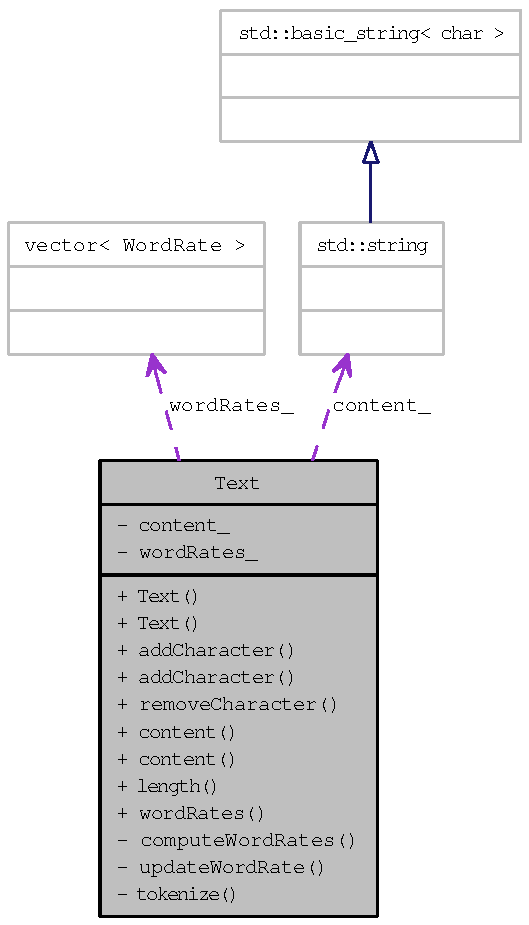
\includegraphics[height=400pt]{class_text__coll__graph}
\end{center}
\end{figure}


\subsection{Detailed Description}
\hyperlink{class_text}{Text} extracted by the recognizer. 

This class stores the text that has been extracted from the press clip during the recognition process. It also keeps the appearance rate of every word in text.

\begin{Desc}
\item[Author:]Eliezer Talón (\href{mailto:elitalon@gmail.com}{\tt elitalon@gmail.com}) \end{Desc}
\begin{Desc}
\item[Date:]2008-10-04 \end{Desc}


Definition at line 25 of file Text.h.\subsection*{Public Member Functions}
\begin{CompactItemize}
\item 
\hyperlink{class_text_b3e26143fccc52699bcc5149cae852bc}{Text} ()
\begin{CompactList}\small\item\em Constructor. \item\end{CompactList}\item 
\hyperlink{class_text_d8c7b52db022f4351e31b2b7609a8180}{Text} (const std::string \&content)
\begin{CompactList}\small\item\em Constructor. \item\end{CompactList}\item 
\hyperlink{class_text_2d49e5c280e205125b149f7777ae30c7}{$\sim$Text} ()
\begin{CompactList}\small\item\em Destructor. \item\end{CompactList}\item 
void \hyperlink{class_text_6e6da63c90af68639adc7dd1336f6bf9}{addCharacter} (const char \&character)
\begin{CompactList}\small\item\em Adds a character to text. \item\end{CompactList}\item 
void \hyperlink{class_text_fdd11ad0c90ca483d4cff3d74a64da9e}{addCharacter} (const char \&character, const unsigned int \&position)
\begin{CompactList}\small\item\em Adds a character to text. \item\end{CompactList}\item 
void \hyperlink{class_text_e04500eeada2a4a3bb00554b32263c52}{removeCharacter} (const unsigned int \&position)
\begin{CompactList}\small\item\em Removes a character from text. \item\end{CompactList}\item 
std::string \hyperlink{class_text_58a34fa2cfd0c240a7517132017b6a83}{content} () const 
\begin{CompactList}\small\item\em Returns the text's content. \item\end{CompactList}\item 
void \hyperlink{class_text_eca454f28010b6b3e7bd0d771b8eaeb2}{content} (const std::string \&content)
\begin{CompactList}\small\item\em Sets the text's content. \item\end{CompactList}\item 
unsigned int \hyperlink{class_text_8d76db538f8617fb8880ba3e4ff3e6a5}{length} () const 
\begin{CompactList}\small\item\em Returns the text's length. \item\end{CompactList}\item 
std::vector$<$ \hyperlink{_word_rate_8h_8cfef8793106ac45a83059bd5573cbb3}{WordRate} $>$ \hyperlink{class_text_1387d9767b65f80355f1bdede26a0f7b}{wordRates} () const 
\begin{CompactList}\small\item\em Returns the appearance rates of every single word in text. \item\end{CompactList}\end{CompactItemize}
\subsection*{Private Member Functions}
\begin{CompactItemize}
\item 
void \hyperlink{class_text_8239e13039bcc1c713f66f1236693706}{computeWordRates} ()
\begin{CompactList}\small\item\em Builds the vector of appearance rates of every word. \item\end{CompactList}\item 
void \hyperlink{class_text_7466754bf64f0c22b291edb2bd14ba99}{updateWordRate} (const std::string \&word\_\-)
\begin{CompactList}\small\item\em Increases by one the number of appearances of a word. \item\end{CompactList}\item 
void \hyperlink{class_text_3fe3daa80386d15a275523b18bde7fd9}{tokenize} (std::vector$<$ std::string $>$ \&tokens\_\-, const std::string \&delimiters\_\-=\char`\"{} ,.$\backslash$n$\backslash$t:;!¡¿?\&/()=$\backslash$\char`\"{}'\char`\"{}) const 
\begin{CompactList}\small\item\em Extracts every word surrounded by a set of delimiters. \item\end{CompactList}\end{CompactItemize}
\subsection*{Private Attributes}
\begin{CompactItemize}
\item 
\hypertarget{class_text_8c5acddb86730d41099c87da7e386f6c}{
std::string \hyperlink{class_text_8c5acddb86730d41099c87da7e386f6c}{content\_\-}}
\label{class_text_8c5acddb86730d41099c87da7e386f6c}

\begin{CompactList}\small\item\em The text's content. \item\end{CompactList}\item 
\hypertarget{class_text_ee3a9a1486714df08c8e73ccb605e729}{
std::vector$<$ \hyperlink{_word_rate_8h_8cfef8793106ac45a83059bd5573cbb3}{WordRate} $>$ \hyperlink{class_text_ee3a9a1486714df08c8e73ccb605e729}{wordRates\_\-}}
\label{class_text_ee3a9a1486714df08c8e73ccb605e729}

\begin{CompactList}\small\item\em A list of appearance rates of every single word in text. \item\end{CompactList}\end{CompactItemize}


\subsection{Constructor \& Destructor Documentation}
\hypertarget{class_text_b3e26143fccc52699bcc5149cae852bc}{
\index{Text@{Text}!Text@{Text}}
\index{Text@{Text}!Text@{Text}}
\subsubsection[Text]{\setlength{\rightskip}{0pt plus 5cm}Text::Text ()}}
\label{class_text_b3e26143fccc52699bcc5149cae852bc}


Constructor. 

Initializes a \hyperlink{class_text}{Text} object with no content

\begin{Desc}
\item[Author:]Eliezer Talón (\href{mailto:elitalon@gmail.com}{\tt elitalon@gmail.com}) \end{Desc}
\begin{Desc}
\item[Date:]2008-10-04 \end{Desc}


Definition at line 19 of file Text.cpp.\hypertarget{class_text_d8c7b52db022f4351e31b2b7609a8180}{
\index{Text@{Text}!Text@{Text}}
\index{Text@{Text}!Text@{Text}}
\subsubsection[Text]{\setlength{\rightskip}{0pt plus 5cm}Text::Text (const std::string \& {\em content})}}
\label{class_text_d8c7b52db022f4351e31b2b7609a8180}


Constructor. 

Initializes a \hyperlink{class_text}{Text} object with the content passed

\begin{Desc}
\item[Parameters:]
\begin{description}
\item[{\em content}]Initial text\end{description}
\end{Desc}
\begin{Desc}
\item[Author:]Eliezer Talón (\href{mailto:elitalon@gmail.com}{\tt elitalon@gmail.com}) \end{Desc}
\begin{Desc}
\item[Date:]2008-10-04 \end{Desc}


Definition at line 34 of file Text.cpp.\hypertarget{class_text_2d49e5c280e205125b149f7777ae30c7}{
\index{Text@{Text}!$\sim$Text@{$\sim$Text}}
\index{$\sim$Text@{$\sim$Text}!Text@{Text}}
\subsubsection[$\sim$Text]{\setlength{\rightskip}{0pt plus 5cm}Text::$\sim$Text ()}}
\label{class_text_2d49e5c280e205125b149f7777ae30c7}


Destructor. 

Destroys a \hyperlink{class_text}{Text} object

\begin{Desc}
\item[Author:]Eliezer Talón (\href{mailto:elitalon@gmail.com}{\tt elitalon@gmail.com}) \end{Desc}
\begin{Desc}
\item[Date:]2008-09-18 \end{Desc}


Definition at line 47 of file Text.cpp.

\subsection{Member Function Documentation}
\hypertarget{class_text_6e6da63c90af68639adc7dd1336f6bf9}{
\index{Text@{Text}!addCharacter@{addCharacter}}
\index{addCharacter@{addCharacter}!Text@{Text}}
\subsubsection[addCharacter]{\setlength{\rightskip}{0pt plus 5cm}void Text::addCharacter (const char \& {\em character})}}
\label{class_text_6e6da63c90af68639adc7dd1336f6bf9}


Adds a character to text. 

The character passed is appended to the end of the text

\begin{Desc}
\item[Parameters:]
\begin{description}
\item[{\em character}]Character to add\end{description}
\end{Desc}
\begin{Desc}
\item[Author:]Eliezer Talón (\href{mailto:elitalon@gmail.com}{\tt elitalon@gmail.com}) \end{Desc}
\begin{Desc}
\item[Date:]2008-10-06 \end{Desc}


Definition at line 89 of file Text.cpp.\hypertarget{class_text_fdd11ad0c90ca483d4cff3d74a64da9e}{
\index{Text@{Text}!addCharacter@{addCharacter}}
\index{addCharacter@{addCharacter}!Text@{Text}}
\subsubsection[addCharacter]{\setlength{\rightskip}{0pt plus 5cm}void Text::addCharacter (const char \& {\em character}, \/  const unsigned int \& {\em position})}}
\label{class_text_fdd11ad0c90ca483d4cff3d74a64da9e}


Adds a character to text. 

The character is inserted within the text at position passed. If the position passed is over the text total length, the character is appended to the end of the text. If th position passed is less than 0, the character is inserted at the beginning of the text.

\begin{Desc}
\item[Parameters:]
\begin{description}
\item[{\em character}]Character to add \item[{\em position}]Position where adding the character to\end{description}
\end{Desc}
\begin{Desc}
\item[Author:]Eliezer Talón (\href{mailto:elitalon@gmail.com}{\tt elitalon@gmail.com}) \end{Desc}
\begin{Desc}
\item[Date:]2008-10-03 \end{Desc}


Definition at line 64 of file Text.cpp.\hypertarget{class_text_e04500eeada2a4a3bb00554b32263c52}{
\index{Text@{Text}!removeCharacter@{removeCharacter}}
\index{removeCharacter@{removeCharacter}!Text@{Text}}
\subsubsection[removeCharacter]{\setlength{\rightskip}{0pt plus 5cm}void Text::removeCharacter (const unsigned int \& {\em position})}}
\label{class_text_e04500eeada2a4a3bb00554b32263c52}


Removes a character from text. 

The character is removed from text at position passed. If the position passed is over the text total length, the last character is removed. If the position passed is less than 0 the first character is removed.

\begin{Desc}
\item[Parameters:]
\begin{description}
\item[{\em position}]Position where removing the character from\end{description}
\end{Desc}
\begin{Desc}
\item[Author:]Eliezer Talón (\href{mailto:elitalon@gmail.com}{\tt elitalon@gmail.com}) \end{Desc}
\begin{Desc}
\item[Date:]2008-10-03 \end{Desc}


Definition at line 105 of file Text.cpp.\hypertarget{class_text_58a34fa2cfd0c240a7517132017b6a83}{
\index{Text@{Text}!content@{content}}
\index{content@{content}!Text@{Text}}
\subsubsection[content]{\setlength{\rightskip}{0pt plus 5cm}std::string Text::content () const}}
\label{class_text_58a34fa2cfd0c240a7517132017b6a83}


Returns the text's content. 

\begin{Desc}
\item[Returns:]The content of the text\end{Desc}
\begin{Desc}
\item[Author:]Eliezer Talón (\href{mailto:elitalon@gmail.com}{\tt elitalon@gmail.com}) \end{Desc}
\begin{Desc}
\item[Date:]2008-10-04 \end{Desc}


Definition at line 129 of file Text.cpp.\hypertarget{class_text_eca454f28010b6b3e7bd0d771b8eaeb2}{
\index{Text@{Text}!content@{content}}
\index{content@{content}!Text@{Text}}
\subsubsection[content]{\setlength{\rightskip}{0pt plus 5cm}void Text::content (const std::string \& {\em content})}}
\label{class_text_eca454f28010b6b3e7bd0d771b8eaeb2}


Sets the text's content. 

\begin{Desc}
\item[Parameters:]
\begin{description}
\item[{\em content}]The content of the text\end{description}
\end{Desc}
\begin{Desc}
\item[Author:]Eliezer Talón (\href{mailto:elitalon@gmail.com}{\tt elitalon@gmail.com}) \end{Desc}
\begin{Desc}
\item[Date:]2008-10-04 \end{Desc}


Definition at line 141 of file Text.cpp.\hypertarget{class_text_8d76db538f8617fb8880ba3e4ff3e6a5}{
\index{Text@{Text}!length@{length}}
\index{length@{length}!Text@{Text}}
\subsubsection[length]{\setlength{\rightskip}{0pt plus 5cm}unsigned int Text::length () const}}
\label{class_text_8d76db538f8617fb8880ba3e4ff3e6a5}


Returns the text's length. 

\begin{Desc}
\item[Returns:]The length of the text\end{Desc}
\begin{Desc}
\item[Author:]Eliezer Talón (\href{mailto:elitalon@gmail.com}{\tt elitalon@gmail.com}) \end{Desc}
\begin{Desc}
\item[Date:]2008-09-29 \end{Desc}


Definition at line 156 of file Text.cpp.\hypertarget{class_text_1387d9767b65f80355f1bdede26a0f7b}{
\index{Text@{Text}!wordRates@{wordRates}}
\index{wordRates@{wordRates}!Text@{Text}}
\subsubsection[wordRates]{\setlength{\rightskip}{0pt plus 5cm}std::vector$<$ {\bf WordRate} $>$ Text::wordRates () const}}
\label{class_text_1387d9767b65f80355f1bdede26a0f7b}


Returns the appearance rates of every single word in text. 

\begin{Desc}
\item[Returns:]A vector with every different word and their appearance rate\end{Desc}
\begin{Desc}
\item[See also:]\hyperlink{_word_rate_8h_8cfef8793106ac45a83059bd5573cbb3}{WordRate}\end{Desc}
\begin{Desc}
\item[Author:]Eliezer Talón (\href{mailto:elitalon@gmail.com}{\tt elitalon@gmail.com}) \end{Desc}
\begin{Desc}
\item[Date:]2008-09-24 \end{Desc}


Definition at line 170 of file Text.cpp.

Referenced by updateWordRate().\hypertarget{class_text_8239e13039bcc1c713f66f1236693706}{
\index{Text@{Text}!computeWordRates@{computeWordRates}}
\index{computeWordRates@{computeWordRates}!Text@{Text}}
\subsubsection[computeWordRates]{\setlength{\rightskip}{0pt plus 5cm}void Text::computeWordRates ()\hspace{0.3cm}{\tt  \mbox{[}private\mbox{]}}}}
\label{class_text_8239e13039bcc1c713f66f1236693706}


Builds the vector of appearance rates of every word. 

This method must be called every time the content changes, since there is no public method for a class user to make it by itself.

\begin{Desc}
\item[Author:]Eliezer Talón (\href{mailto:elitalon@gmail.com}{\tt elitalon@gmail.com}) \end{Desc}
\begin{Desc}
\item[Date:]2008-10-04 \end{Desc}


Definition at line 208 of file Text.cpp.

Referenced by addCharacter(), content(), removeCharacter(), and Text().\hypertarget{class_text_7466754bf64f0c22b291edb2bd14ba99}{
\index{Text@{Text}!updateWordRate@{updateWordRate}}
\index{updateWordRate@{updateWordRate}!Text@{Text}}
\subsubsection[updateWordRate]{\setlength{\rightskip}{0pt plus 5cm}void Text::updateWordRate (const std::string \& {\em word})\hspace{0.3cm}{\tt  \mbox{[}private\mbox{]}}}}
\label{class_text_7466754bf64f0c22b291edb2bd14ba99}


Increases by one the number of appearances of a word. 

\begin{Desc}
\item[Parameters:]
\begin{description}
\item[{\em word}]Word whose appearance rate must be update\end{description}
\end{Desc}
\begin{Desc}
\item[Author:]Eliezer Talón (\href{mailto:elitalon@gmail.com}{\tt elitalon@gmail.com}) \end{Desc}
\begin{Desc}
\item[Date:]2008-10-04 \end{Desc}


Definition at line 182 of file Text.cpp.

Referenced by computeWordRates().\hypertarget{class_text_3fe3daa80386d15a275523b18bde7fd9}{
\index{Text@{Text}!tokenize@{tokenize}}
\index{tokenize@{tokenize}!Text@{Text}}
\subsubsection[tokenize]{\setlength{\rightskip}{0pt plus 5cm}void Text::tokenize (std::vector$<$ std::string $>$ \& {\em tokens}, \/  const std::string \& {\em delimiters} = {\tt \char`\"{}~,.$\backslash$n$\backslash$t:;!¡¿?\&/()=$\backslash$\char`\"{}'\char`\"{}}) const\hspace{0.3cm}{\tt  \mbox{[}private\mbox{]}}}}
\label{class_text_3fe3daa80386d15a275523b18bde7fd9}


Extracts every word surrounded by a set of delimiters. 

\begin{Desc}
\item[Parameters:]
\begin{description}
\item[\mbox{$\rightarrow$} {\em tokens}]Vector where storing the words found to \item[{\em delimiters}]Characters that may delimiter a valid word\end{description}
\end{Desc}
\begin{Desc}
\item[Author:]Eliezer Talón (\href{mailto:elitalon@gmail.com}{\tt elitalon@gmail.com}) \end{Desc}
\begin{Desc}
\item[Date:]2008-10-04 \end{Desc}


Definition at line 232 of file Text.cpp.

Referenced by computeWordRates().

The documentation for this class was generated from the following files:\begin{CompactItemize}
\item 
\hyperlink{_text_8h}{Text.h (125)}\item 
\hyperlink{_text_8cpp}{Text.cpp (125)}\end{CompactItemize}

\chapter{File Documentation}
\hypertarget{_clip_8cpp}{
\section{Clip.cpp File Reference}
\label{_clip_8cpp}\index{Clip.cpp(128)@{Clip.cpp(128)}}
}


\subsection{Detailed Description}
Implementation of the class \hyperlink{class_clip}{Clip}. 



Definition in file \hyperlink{_clip_8cpp-source}{Clip.cpp}.

{\tt \#include \char`\"{}Clip.h\char`\"{}}\par
{\tt \#include \char`\"{}NessieException.h\char`\"{}}\par


Include dependency graph for Clip.cpp:\nopagebreak
\begin{figure}[H]
\begin{center}
\leavevmode
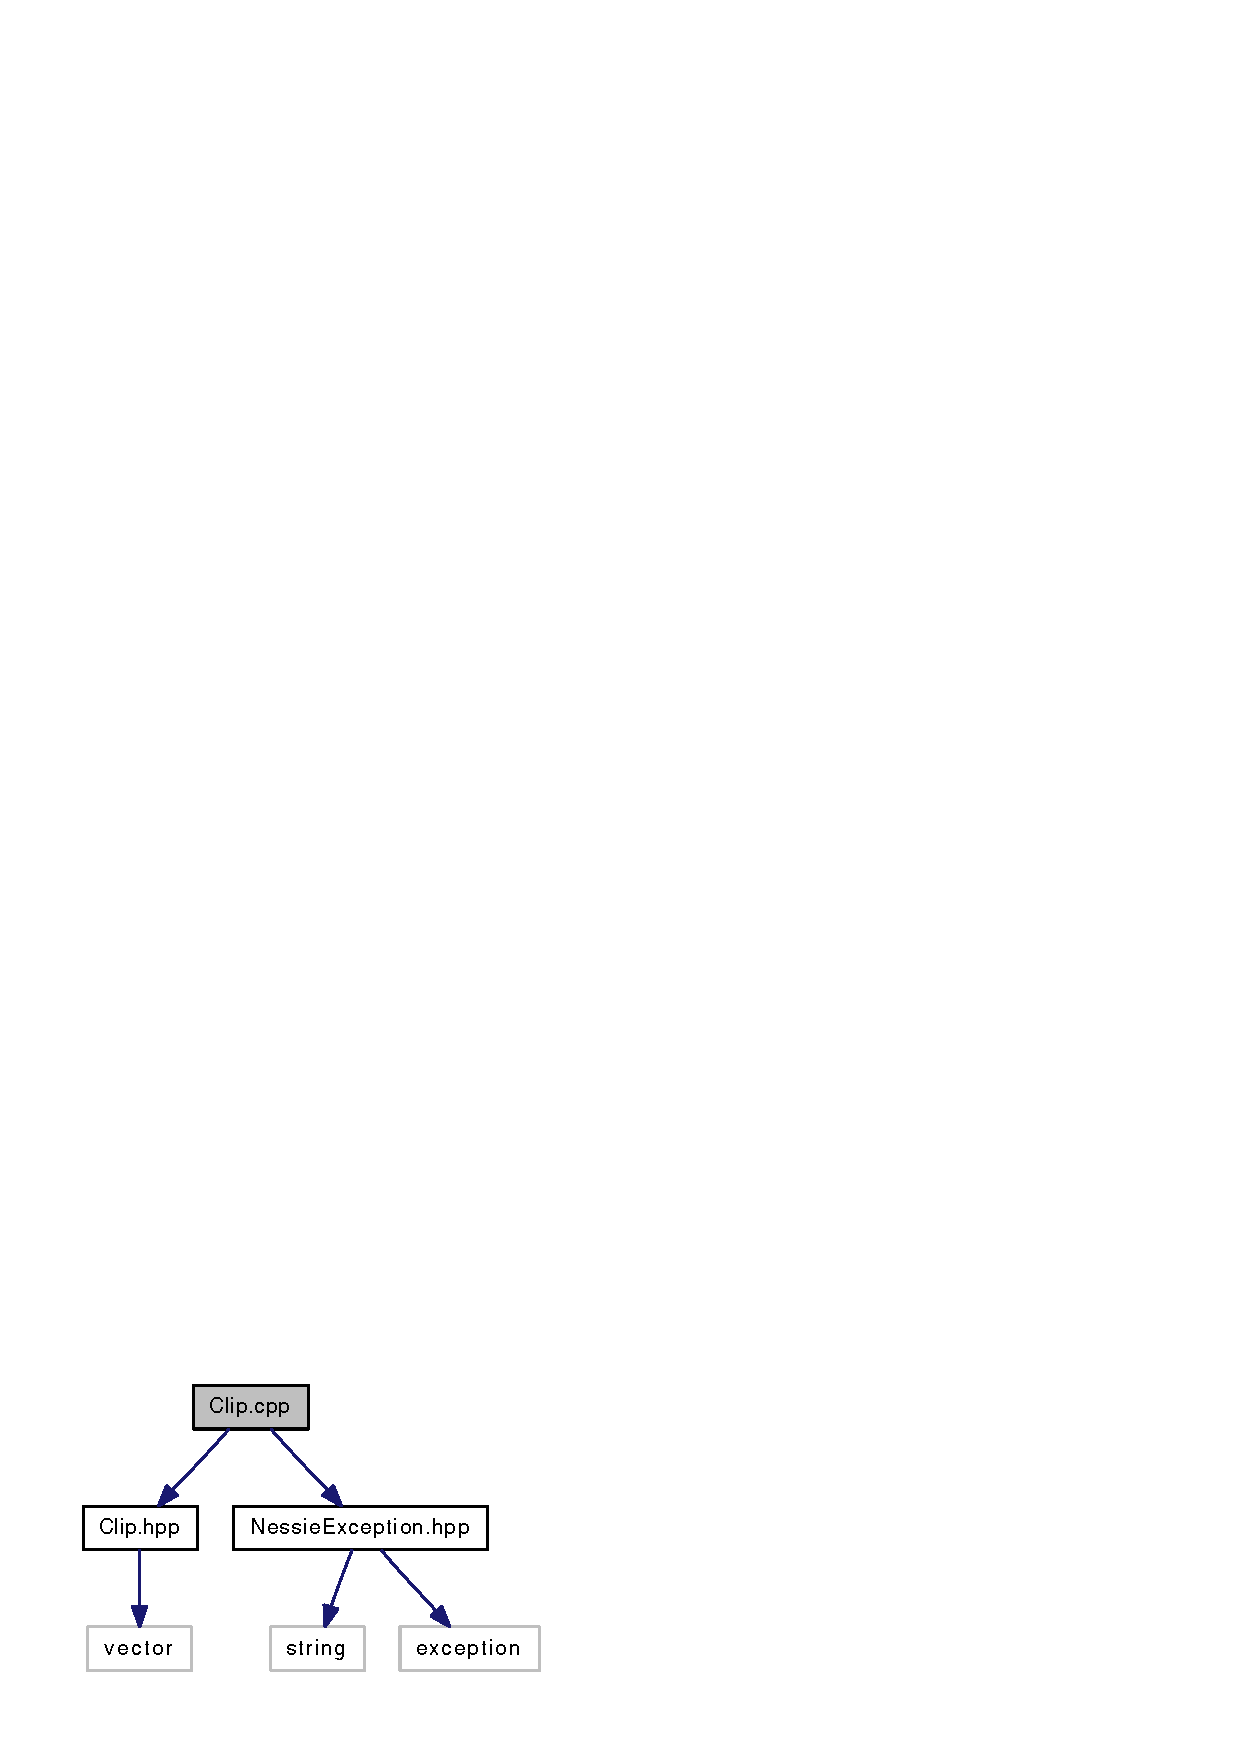
\includegraphics[width=127pt]{_clip_8cpp__incl}
\end{center}
\end{figure}

\hypertarget{_clip_8h}{
\section{Clip.h File Reference}
\label{_clip_8h}\index{Clip.h(136)@{Clip.h(136)}}
}


\subsection{Detailed Description}
Declaration of the class \hyperlink{class_clip}{Clip}. 



Definition in file \hyperlink{_clip_8h-source}{Clip.h}.

{\tt \#include $<$vector$>$}\par


Include dependency graph for Clip.h:\nopagebreak
\begin{figure}[H]
\begin{center}
\leavevmode
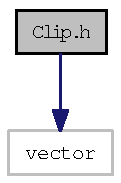
\includegraphics[width=47pt]{_clip_8h__incl}
\end{center}
\end{figure}


This graph shows which files directly or indirectly include this file:\nopagebreak
\begin{figure}[H]
\begin{center}
\leavevmode
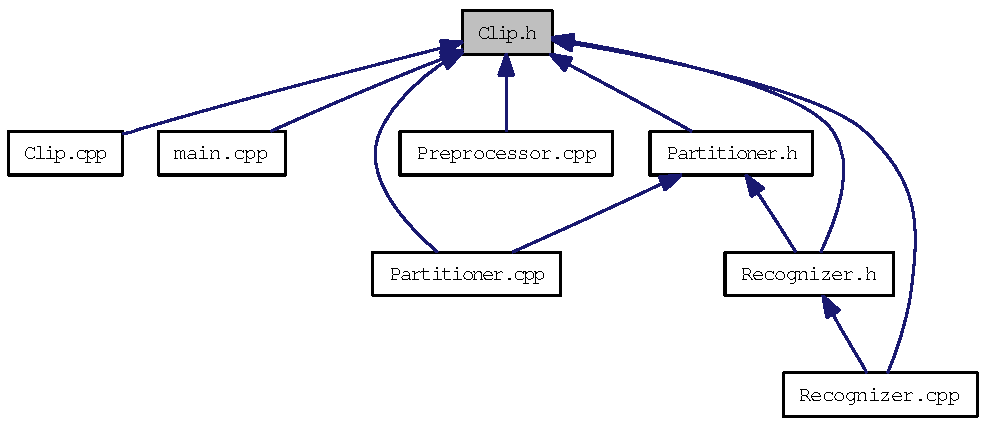
\includegraphics[width=231pt]{_clip_8h__dep__incl}
\end{center}
\end{figure}
\subsection*{Data Structures}
\begin{CompactItemize}
\item 
class \hyperlink{class_clip}{Clip}
\begin{CompactList}\small\item\em Press clip where the recognizer has to extract the text from. \item\end{CompactList}\end{CompactItemize}

\hypertarget{_nessie_exception_8cpp}{
\section{NessieException.cpp File Reference}
\label{_nessie_exception_8cpp}\index{NessieException.cpp@{NessieException.cpp}}
}


\subsection{Detailed Description}
Implementation of class \hyperlink{class_nessie_exception}{NessieException}. 



Definition in file \hyperlink{_nessie_exception_8cpp-source}{NessieException.cpp}.

{\tt \#include \char`\"{}NessieException.h\char`\"{}}\par


Include dependency graph for NessieException.cpp:\nopagebreak
\begin{figure}[H]
\begin{center}
\leavevmode
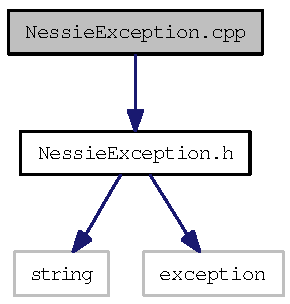
\includegraphics[width=83pt]{_nessie_exception_8cpp__incl}
\end{center}
\end{figure}

\hypertarget{_nessie_exception_8h}{
\section{NessieException.h File Reference}
\label{_nessie_exception_8h}\index{NessieException.h(114)@{NessieException.h(114)}}
}


\subsection{Detailed Description}
Declaration of class \hyperlink{class_nessie_exception}{NessieException}. 



Definition in file \hyperlink{_nessie_exception_8h-source}{NessieException.h}.

{\tt \#include $<$string$>$}\par


Include dependency graph for NessieException.h:\nopagebreak
\begin{figure}[H]
\begin{center}
\leavevmode
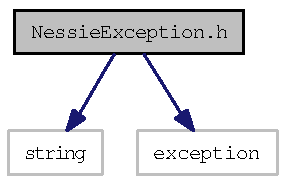
\includegraphics[width=77pt]{_nessie_exception_8h__incl}
\end{center}
\end{figure}


This graph shows which files directly or indirectly include this file:\nopagebreak
\begin{figure}[H]
\begin{center}
\leavevmode
\includegraphics[width=227pt]{_nessie_exception_8h__dep__incl}
\end{center}
\end{figure}
\subsection*{Data Structures}
\begin{CompactItemize}
\item 
class \hyperlink{class_nessie_exception}{NessieException}
\begin{CompactList}\small\item\em Exception raised by a Nessie OCR object. \item\end{CompactList}\end{CompactItemize}

\hypertarget{_pixel_8cpp}{
\section{Pixel.cpp File Reference}
\label{_pixel_8cpp}\index{Pixel.cpp(132)@{Pixel.cpp(132)}}
}


\subsection{Detailed Description}
Implementation of the class \hyperlink{class_pixel}{Pixel}. 



Definition in file \hyperlink{_pixel_8cpp-source}{Pixel.cpp}.

{\tt \#include \char`\"{}Pixel.h\char`\"{}}\par


Include dependency graph for Pixel.cpp:\nopagebreak
\begin{figure}[H]
\begin{center}
\leavevmode
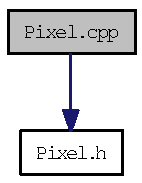
\includegraphics[width=52pt]{_pixel_8cpp__incl}
\end{center}
\end{figure}

\hypertarget{_pixel_8h}{
\section{Pixel.h File Reference}
\label{_pixel_8h}\index{Pixel.h(114)@{Pixel.h(114)}}
}


\subsection{Detailed Description}
Declaration of class \hyperlink{class_pixel}{Pixel}. 



Definition in file \hyperlink{_pixel_8h-source}{Pixel.h}.

{\tt \#include \char`\"{}Colorspace.h\char`\"{}}\par
{\tt \#include $<$Magick++.h$>$}\par


Include dependency graph for Pixel.h:\nopagebreak
\begin{figure}[H]
\begin{center}
\leavevmode
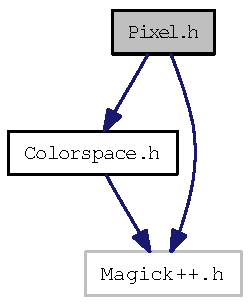
\includegraphics[width=77pt]{_pixel_8h__incl}
\end{center}
\end{figure}


This graph shows which files directly or indirectly include this file:\nopagebreak
\begin{figure}[H]
\begin{center}
\leavevmode
\includegraphics[width=408pt]{_pixel_8h__dep__incl}
\end{center}
\end{figure}
\subsection*{Data Structures}
\begin{CompactItemize}
\item 
class \hyperlink{class_pixel}{Pixel}
\begin{CompactList}\small\item\em Information about an image pixel. \item\end{CompactList}\end{CompactItemize}

\hypertarget{_preprocessor_8cpp}{
\subsection{Preprocessor.cpp File Reference}
\label{_preprocessor_8cpp}\index{Preprocessor.cpp(166)@{Preprocessor.cpp(166)}}
}
Definition of \hyperlink{class_preprocessor}{Preprocessor} class.  


{\tt \#include \char`\"{}Preprocessor.hpp\char`\"{}}\par
{\tt \#include \char`\"{}Clip.hpp\char`\"{}}\par
{\tt \#include \char`\"{}boost/timer.hpp\char`\"{}}\par
{\tt \#include $<$cmath$>$}\par


Include dependency graph for Preprocessor.cpp:\nopagebreak
\begin{figure}[H]
\begin{center}
\leavevmode
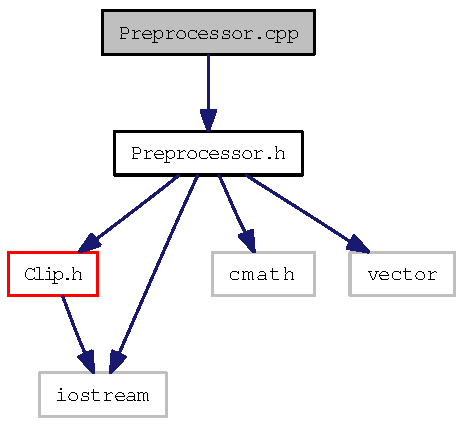
\includegraphics[width=199pt]{_preprocessor_8cpp__incl}
\end{center}
\end{figure}


\subsubsection{Detailed Description}
Definition of \hyperlink{class_preprocessor}{Preprocessor} class. 


\hypertarget{_preprocessor_8h}{
\section{Preprocessor.h File Reference}
\label{_preprocessor_8h}\index{Preprocessor.h(125)@{Preprocessor.h(125)}}
}


\subsection{Detailed Description}
Declaration of class \hyperlink{class_preprocessor}{Preprocessor}. 



Definition in file \hyperlink{_preprocessor_8h-source}{Preprocessor.h}.



This graph shows which files directly or indirectly include this file:\nopagebreak
\begin{figure}[H]
\begin{center}
\leavevmode
\includegraphics[width=164pt]{_preprocessor_8h__dep__incl}
\end{center}
\end{figure}
\subsection*{Data Structures}
\begin{CompactItemize}
\item 
class \hyperlink{class_preprocessor}{Preprocessor}
\begin{CompactList}\small\item\em \hyperlink{class_preprocessor}{Preprocessor} of the OCR process. \item\end{CompactList}\end{CompactItemize}

\hypertarget{_statistics_8cpp}{
\subsection{Statistics.cpp File Reference}
\label{_statistics_8cpp}\index{Statistics.cpp(162)@{Statistics.cpp(162)}}
}
Definition of \hyperlink{class_statistics}{Statistics} class.  


{\tt \#include \char`\"{}Statistics.hpp\char`\"{}}\par


Include dependency graph for Statistics.cpp:\nopagebreak
\begin{figure}[H]
\begin{center}
\leavevmode
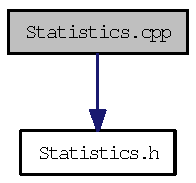
\includegraphics[width=65pt]{_statistics_8cpp__incl}
\end{center}
\end{figure}


\subsubsection{Detailed Description}
Definition of \hyperlink{class_statistics}{Statistics} class. 


\hypertarget{_statistics_8h}{
\section{Statistics.h File Reference}
\label{_statistics_8h}\index{Statistics.h(136)@{Statistics.h(136)}}
}


\subsection{Detailed Description}
Declaration of the class \hyperlink{class_statistics}{Statistics}. 



Definition in file \hyperlink{_statistics_8h-source}{Statistics.h}.



This graph shows which files directly or indirectly include this file:\nopagebreak
\begin{figure}[H]
\begin{center}
\leavevmode
\includegraphics[width=140pt]{_statistics_8h__dep__incl}
\end{center}
\end{figure}
\subsection*{Data Structures}
\begin{CompactItemize}
\item 
class \hyperlink{class_statistics}{Statistics}
\begin{CompactList}\small\item\em \hyperlink{class_statistics}{Statistics} about the text recognition process. \item\end{CompactList}\end{CompactItemize}

\hypertarget{_text_8cpp}{
\section{Text.cpp File Reference}
\label{_text_8cpp}\index{Text.cpp(132)@{Text.cpp(132)}}
}


\subsection{Detailed Description}
Implementation of the class \hyperlink{class_text}{Text}. 



Definition in file \hyperlink{_text_8cpp-source}{Text.cpp}.

{\tt \#include \char`\"{}Text.h\char`\"{}}\par
{\tt \#include $<$algorithm$>$}\par
{\tt \#include $<$string$>$}\par
{\tt \#include $<$vector$>$}\par


Include dependency graph for Text.cpp:\nopagebreak
\begin{figure}[H]
\begin{center}
\leavevmode
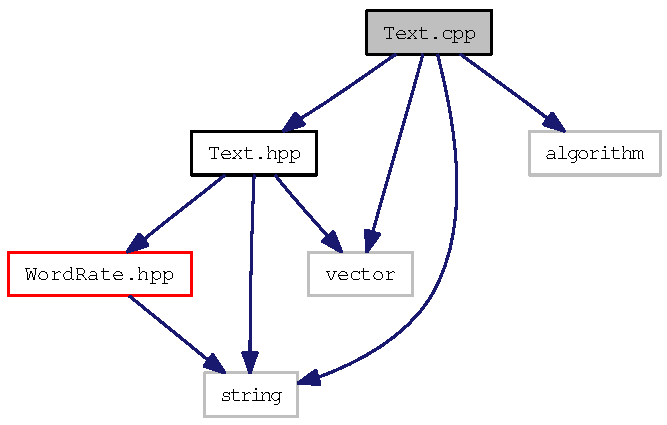
\includegraphics[width=172pt]{_text_8cpp__incl}
\end{center}
\end{figure}

\hypertarget{_text_8h}{
\section{Text.h File Reference}
\label{_text_8h}\index{Text.h(116)@{Text.h(116)}}
}


\subsection{Detailed Description}
Declaration of class \hyperlink{class_text}{Text}. 



Definition in file \hyperlink{_text_8h-source}{Text.h}.

{\tt \#include \char`\"{}WordRate.h\char`\"{}}\par
{\tt \#include \char`\"{}FontProportionality.h\char`\"{}}\par
{\tt \#include \char`\"{}Style.h\char`\"{}}\par
{\tt \#include $<$string$>$}\par
{\tt \#include $<$vector$>$}\par
{\tt \#include $<$algorithm$>$}\par


Include dependency graph for Text.h:\nopagebreak
\begin{figure}[H]
\begin{center}
\leavevmode
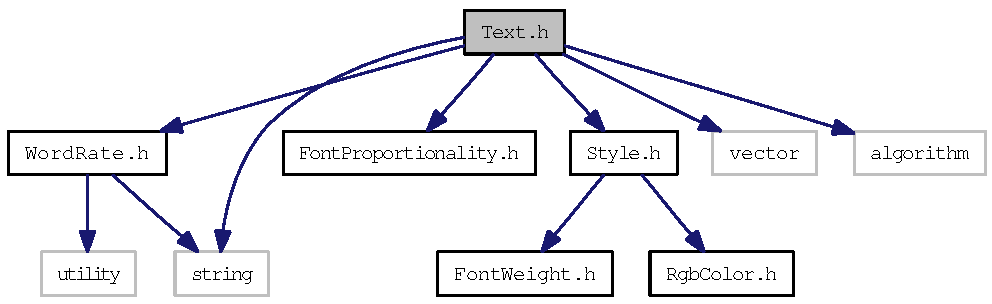
\includegraphics[width=256pt]{_text_8h__incl}
\end{center}
\end{figure}


This graph shows which files directly or indirectly include this file:\nopagebreak
\begin{figure}[H]
\begin{center}
\leavevmode
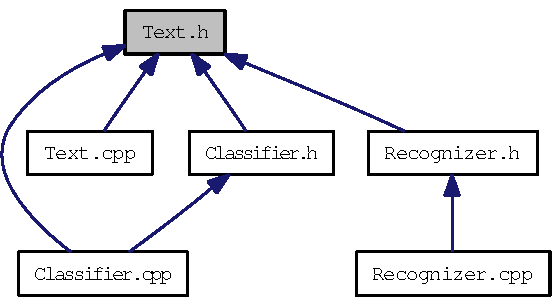
\includegraphics[width=122pt]{_text_8h__dep__incl}
\end{center}
\end{figure}
\subsection*{Data Structures}
\begin{CompactItemize}
\item 
class \hyperlink{class_text}{Text}
\begin{CompactList}\small\item\em \hyperlink{class_text}{Text} extracted from the clip by the recognizer. \item\end{CompactList}\end{CompactItemize}

\hypertarget{_word_rate_8h}{
\section{WordRate.h File Reference}
\label{_word_rate_8h}\index{WordRate.h(125)@{WordRate.h(125)}}
}


\subsection{Detailed Description}
Declaration of custom type WordRate. 



Definition in file \hyperlink{_word_rate_8h-source}{WordRate.h}.

{\tt \#include $<$utility$>$}\par
{\tt \#include $<$string$>$}\par


Include dependency graph for WordRate.h:\nopagebreak
\begin{figure}[H]
\begin{center}
\leavevmode
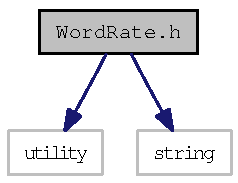
\includegraphics[width=75pt]{_word_rate_8h__incl}
\end{center}
\end{figure}


This graph shows which files directly or indirectly include this file:\nopagebreak
\begin{figure}[H]
\begin{center}
\leavevmode
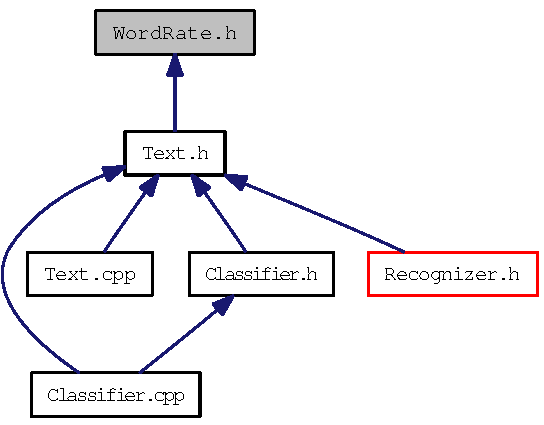
\includegraphics[width=148pt]{_word_rate_8h__dep__incl}
\end{center}
\end{figure}
\subsection*{Typedefs}
\begin{CompactItemize}
\item 
typedef std::pair$<$ std::string, unsigned int $>$ \hyperlink{_word_rate_8h_8cfef8793106ac45a83059bd5573cbb3}{WordRate}
\begin{CompactList}\small\item\em Appearance rate of a word. \item\end{CompactList}\end{CompactItemize}


\subsection{Typedef Documentation}
\hypertarget{_word_rate_8h_8cfef8793106ac45a83059bd5573cbb3}{
\index{WordRate.h@{WordRate.h}!WordRate@{WordRate}}
\index{WordRate@{WordRate}!WordRate.h@{WordRate.h}}
\subsubsection[WordRate]{\setlength{\rightskip}{0pt plus 5cm}typedef std::pair$<$std::string, unsigned int$>$ {\bf WordRate}}}
\label{_word_rate_8h_8cfef8793106ac45a83059bd5573cbb3}


Appearance rate of a word. 

This pair keeps the number of appearances of a word in a text

\begin{Desc}
\item[Author:]Eliezer Talón (\href{mailto:elitalon@gmail.com}{\tt elitalon@gmail.com}) \end{Desc}
\begin{Desc}
\item[Date:]2008-09-19 \end{Desc}


Definition at line 21 of file WordRate.h.
\printindex
\end{document}
